\documentclass[12pt]{article}
\setcounter{tocdepth}{4}
 \setcounter{secnumdepth}{4}
\renewcommand{\labelenumii}{\theenumii}
\renewcommand{\theenumii}{\theenumi.\arabic{enumii}.}
\usepackage[utf8]{inputenc}
%\usepackage[T1]{fontenc}

\usepackage{geometry}
\geometry{a4paper}
\usepackage{graphicx}
\usepackage{float}
\usepackage[italian]{babel}

\linespread{1.2}
\setlength{\parindent}{0pt}

\usepackage[T1]{fontenc}
\usepackage{inconsolata}

\usepackage{color}
\definecolor{bluekeywords}{rgb}{0.13,0.13,1}
\definecolor{greencomments}{rgb}{0,0.5,0}
\definecolor{redstrings}{rgb}{0.9,0,0}

\usepackage{listings}
\lstset{language=[Sharp]C,
  showspaces=false,
  showtabs=false,
  breaklines=true,
  showstringspaces=false,
  breakatwhitespace=true,
  escapeinside={(*@}{@*)},
  commentstyle=\color{greencomments},
  keywordstyle=\color{bluekeywords},
  stringstyle=\color{redstrings},
  basicstyle={\footnotesize\ttfamily},   
}


\definecolor{lightgray}{rgb}{0.95, 0.95, 0.95}
\definecolor{darkgray}{rgb}{0.4, 0.4, 0.4}
%\definecolor{purple}{rgb}{0.65, 0.12, 0.82}
\definecolor{editorGray}{rgb}{0.95, 0.95, 0.95}
\definecolor{editorOcher}{rgb}{1, 0.5, 0} % #FF7F00 -> rgb(239, 169, 0)
\definecolor{editorGreen}{rgb}{0, 0.5, 0} % #007C00 -> rgb(0, 124, 0)
\definecolor{orange}{rgb}{1,0.45,0.13}		
\definecolor{olive}{rgb}{0.17,0.59,0.20}
\definecolor{brown}{rgb}{0.69,0.31,0.31}
\definecolor{purple}{rgb}{0.38,0.18,0.81}
\definecolor{lightblue}{rgb}{0.1,0.57,0.7}
\definecolor{lightred}{rgb}{1,0.4,0.5}
\usepackage{upquote}
\usepackage{listings}
% CSS
\lstdefinelanguage{CSS}{
  keywords={color,background-image:,margin,padding,font,weight,display,position,top,left,right,bottom,list,style,border,size,white,space,min,width, transition:, transform:, transition-property, transition-duration, transition-timing-function},	
  sensitive=true,
  morecomment=[l]{//},
  morecomment=[s]{/*}{*/},
  morestring=[b]',
  morestring=[b]",
  alsoletter={:},
  alsodigit={-}
}

% JavaScript
\lstdefinelanguage{JavaScript}{
  morekeywords={typeof, new, true, false, catch, function, return, null, catch, switch, var, if, in, while, do, else, case, break},
  morecomment=[s]{/*}{*/},
  morecomment=[l]//,
  morestring=[b]",
  morestring=[b]'
}

\lstdefinelanguage{HTML5}{
  language=html,
  sensitive=true,	
  alsoletter={<>=-},	
  morecomment=[s]{<!-}{-->},
  tag=[s],
  otherkeywords={
  % General
  >,
  % Standard tags
	<!DOCTYPE,
  </html, <html, <head, <title, </title, <style, </style, <link, </head, <meta, />,
<agm-info-window, </agm-info-window, <agm-marker, </agm-marker, <agm-map, </agm-map, <app-marker-detail, </app-marker-detail
	% body
	</body, <body,
	% Divs
	</div, <div, </div>, 
	% Paragraphs
	</p, <p, </p>,
	% scripts
	</script, <script,
  % More tags...
  <canvas, /canvas>, <svg, <rect, <animateTransform, </rect>, </svg>, <video, <source, <iframe, </iframe>, </video>, <image, </image>, <header, </header, <article, </article
  },
  ndkeywords={
  % General
  =,
  % HTML attributes
  charset=, src=, id=, width=, height=, style=, type=, rel=, href=, latitude=, longitude=
  % SVG attributes
  fill=, attributeName=, begin=, dur=, from=, to=, poster=, controls=, x=, y=, repeatCount=, xlink:href=,
  % properties
  margin:, padding:, background-image:, border:, top:, left:, position:, width:, height:, margin-top:, margin-bottom:, font-size:, line-height:,
	% CSS3 properties
  transform:, -moz-transform:, -webkit-transform:,
  animation:, -webkit-animation:,
  transition:,  transition-duration:, transition-property:, transition-timing-function:,
  }
}

\lstdefinestyle{htmlcssjs} {%
  % General design
%  backgroundcolor=\color{editorGray},
  basicstyle={\footnotesize\ttfamily},   
  % line-numbers
  % Code design
  identifierstyle=\color{black},
  keywordstyle=\color{blue}\bfseries,
  ndkeywordstyle=\color{editorGreen}\bfseries,
  stringstyle=\color{editorOcher}\ttfamily,
  commentstyle=\color{brown}\ttfamily,
  % Code
  language=HTML5,
  alsolanguage=JavaScript,
  alsodigit={.:;},	
  tabsize=2,
  showtabs=false,
  showspaces=false,
  showstringspaces=false,
  extendedchars=true,
  breaklines=true,
}
%
\lstdefinestyle{py} {%
language=python,
literate=%
*{0}{{{\color{lightred}0}}}1
{1}{{{\color{lightred}1}}}1
{2}{{{\color{lightred}2}}}1
{3}{{{\color{lightred}3}}}1
{4}{{{\color{lightred}4}}}1
{5}{{{\color{lightred}5}}}1
{6}{{{\color{lightred}6}}}1
{7}{{{\color{lightred}7}}}1
{8}{{{\color{lightred}8}}}1
{9}{{{\color{lightred}9}}}1,
basicstyle=\footnotesize\ttfamily, % Standardschrift
numbers=left,               % Ort der Zeilennummern
%numberstyle=\tiny,          % Stil der Zeilennummern
%stepnumber=2,               % Abstand zwischen den Zeilennummern
numbersep=5pt,              % Abstand der Nummern zum Text
tabsize=4,                  % Groesse von Tabs
extendedchars=true,         %
breaklines=true,            % Zeilen werden Umgebrochen
keywordstyle=\color{blue}\bfseries,
frame=b,
commentstyle=\color{brown}\itshape,
stringstyle=\color{editorOcher}\ttfamily, % Farbe der String
showspaces=false,           % Leerzeichen anzeigen ?
showtabs=false,             % Tabs anzeigen ?
xleftmargin=17pt,
framexleftmargin=17pt,
framexrightmargin=5pt,
framexbottommargin=4pt,
%backgroundcolor=\color{lightgray},
showstringspaces=false,      % Leerzeichen in Strings anzeigen ?
}%
%


\begin{document}

%----------------------------------------------------------------------------------------
%	TITOLO
%----------------------------------------------------------------------------------------

\begin{titlepage}

\newcommand{\HRule}{\rule{\linewidth}{0.5mm}}

\center

\textsc{\Large Relazione di progetto di "Smart City e Tecnologie Mobili"}\\[0.5cm]

\HRule \\[0.4cm]
{ \huge \bfseries Smart Public Restrooms }\\[0.4cm]
\HRule \\[1.5cm]

\vfill

\begin{flushleft}
\emph{Numero del gruppo: 60}\\[1cm]
\emph{Componenti del gruppo: \textit{Stefano Belli}; \textit{Andrea Vecchiotti}}\\[3cm]
\end{flushleft}



\end{titlepage}

%----------------------------------------------------------------------------------------
%	INDICE
%----------------------------------------------------------------------------------------

\tableofcontents

\newpage

%----------------------------------------------------------------------------------------
%	INTRODUZIONE
%----------------------------------------------------------------------------------------

\section{Introduzione}
La possibilità di usufruire di servizi igienici in luoghi pubblici viene percepita al giorno d'oggi come un diritto da parte del singolo cittadino, che si aspetta puntalmente di trovare un servizio funzionante, pulito e facilmente accessibile.\\
Oltre che per una questione di pubblico decoro, le aziende (o enti) sono obbligate per legge\cite{articolo1} a fornire servizi igienici ai propri clienti/dipendenti.\\
Inevitabilmente, tuttavia, la loro manutenzione può incidere in maniera rilevante sul bilancio aziendale annuale; sebbene in alcune realtà tale costo sia tutto sommato contenuto, in altre può essere piuttosto ingente (si pensi ad esempio al caso di \textit{Trenitalia} e a quanti milioni di viaggiatori utilizzano i servizi igienici gratuiti sparsi per le stazioni italiane).\\
%parlare che ogni bagno viene gestito localmente..
\\\\
In questa relazione presentiamo \textit{Smart Public Restroom}, una soluzione capace di contenere i costi operativi e di mantenimento dei bagni pubblici e di incrementare la percezione del servizio da parte degli utenti.\\
Nel dettaglio, \textit{Smart Public Restroom} prevede:
\begin{itemize}
	\item L'installazione di un sistema di monitoraggio per ognuno dei servizi igienici del cliente, capace (grazie a una serie di microcontrollori e trasduttori) di individuare rapidamente le problematiche che riscontrano negli impianti (come ad esempio il malfunzionamento di una luce, l'esaurimento del sapone sanitario o il riempimento del bidone della spazzatura).\\
	Tale sistema si configurerà di una parte \textit{locale} a basso costo composta da alcuni sensori (come fotoresistenze, sensori di pressione ecc.) e microcontrollori (come \textit{arduino} e \textit{Raspberry Pi}) e da una parte \textit{Manager} composta da una SPA scritta in \textit{Angular} e \textit{asp.net core}.
	\item Il rilascio di un'applicazione PWA \textit{Consumer} (scritta anch'essa in \textit{Angular}) studiata per dare la possibilità di segnalare eventuali problematiche riscontrate negli impianti e di individuare (grazie a una mappa interattiva) il più vicino servizio igienico.\\
\end{itemize}
Ovviamente, questa tipologia di soluzione è adeguata a una gestione centralizzata dei servizi igienici forniti dall'azienda/ente: avere del personale dedicato alla riparazione e alla pulizia degli impianti (ad esempio su scala nazionale) permetterà di sfruttare appieno le potenzialità di \textit{Smart Public Restroom}.\\\\
Da un punto di vista puramente didattico i punti di interesse di questo progetto sono molteplici:
\begin{itemize}
\item È stato realizzato un sistema di monitoraggio a basso livello con hardware economico e di facile reperibilità.\\
Ogni impianto composto da tre celle, infatti, impiega circa 100€ di hardware e utilizza sensori e microcontrollori molto comuni nel settore.
\item Alcune scelte progettuali sono state motivate in un'ottica di reale, riproducendo motivazioni che si possono realmente trovare in un contesto aziendale medio-piccolo (a tal fine, si è ipotizzato che lo sviluppo dell'applicazione sia stato dato in \textit{outsourcing} a un azienda IT).\\
A titolo di esempio, l'applicazione \textit{Consumer} è stata studiata come PWA sia perché è coerente con il trend tecnologico del settore sia perché comportava un notevole risparmio in termini di risorse per l'azienda.\\
Coerentemente, questa ambientazione reale non ha trascurato i possibili impieghi lavorativi correlati al progetto: sono stati ipotizzate delle figure professionali (come il \textit{configuratore} o il \textit{manager}) che verranno collocate all'interno di questo caso di studio.
\item Anche la scelta delle tecnologie utilizzate non è stata casuale o motivata semplicemente da motivazioni di studio: dove possibile è stato sempre individuato il miglior compromesso tra novità tecnologica e relativa affidabilità.\\
Ad esempio, per il \textit{frontend} è stato utilizzato \textit{Angular} e \textit{ASP.NET Core}, due framework al momento molto popolari, recenti e supportati direttamente da case madre come \textit{Google} e \textit{Microsoft}.
\end{itemize}

%La relazione è strutturata nelle seguenti parti:
% nel primo capitolo saranno definiti e analizzati i requisiti del sistema
%che si intende realizzare;
% nel secondo capitolo sarà descritta l’architettura del progetto, derivata
%dall’analisi dei requisiti, oltre allo schema di deployment;
% nel terzo capitolo verrà illustrata l’implementazione realizzata;
% nel quarto capitolo saranno presentati i test effettuati.
%Per la sua adozione
%A nostro parere, la soluzione è quella di adottare un sistema centralizzato di gestione e reportistica dei servizi pubblici, capace di individuare rapidamente le problematiche che riscontrano negli impianti e razionalizzare così le risorse assegnate.\\
%\textit{Smart Public Restrooms} è la soluzione che riteniamo essere in grado di rispondere a tali specifiche; un sistema a basso costo hardware (si può stimare che per ogni impianto vi sia un costo hardware cbe va dai 100 ai 300€) e di facile utilizzo per i gestori.
%capace di migliorare sia la qualità del servizio che i costi di gestione per le aziende 
\newpage

%----------------------------------------------------------------------------------------
%	STATO DELL'ARTE
%----------------------------------------------------------------------------------------

\section{Stato dell'arte}

La letteratura accademica annovera un discreto numero di pubblicazioni riguardanti l'integrazione di sistemi  \textit{smart} di toilette.\\\\
A titolo di esempio, \textit{Koa et al.}\cite{KooBathroom} presentano una soluzione di informatizzazione di un bagno privato di un appartamento, grazie all'utilizzo di una serie di sensori suddivisi in "nodi" logici.\\
Sebbene l'architettura proposta a livello di sensoristica non sia direttamente comparabile a quella presentata in questo documento (vengono infatti adottati dei trasduttori completamente differenti) si possono individuare delle analogie con la suddivisione logica del sistema.\\
Viene infatti teorizzata la creazione di un nodo di comunicazione per ogni parte suddivisibile della struttura: uno per il settore doccia, uno per il pavimento ecc.
Ognuno di questi nodi verrà connesso a un \textit{Gateway} (un \textit{arduino Yun}) tramite trasmittenti \textit{ZigBee}.
\textit{Smart Public Restrooms} adotta una suddivisione logica molto simile simile: ogni cella singola celle e la struttura nel suo insieme vengono gestite da un singolo \textit{Arduino}, che invia i dati a un \textit{Raspberry Pi} operante da \textit{Gateway}.\\\\
\begin{figure}[h!]
  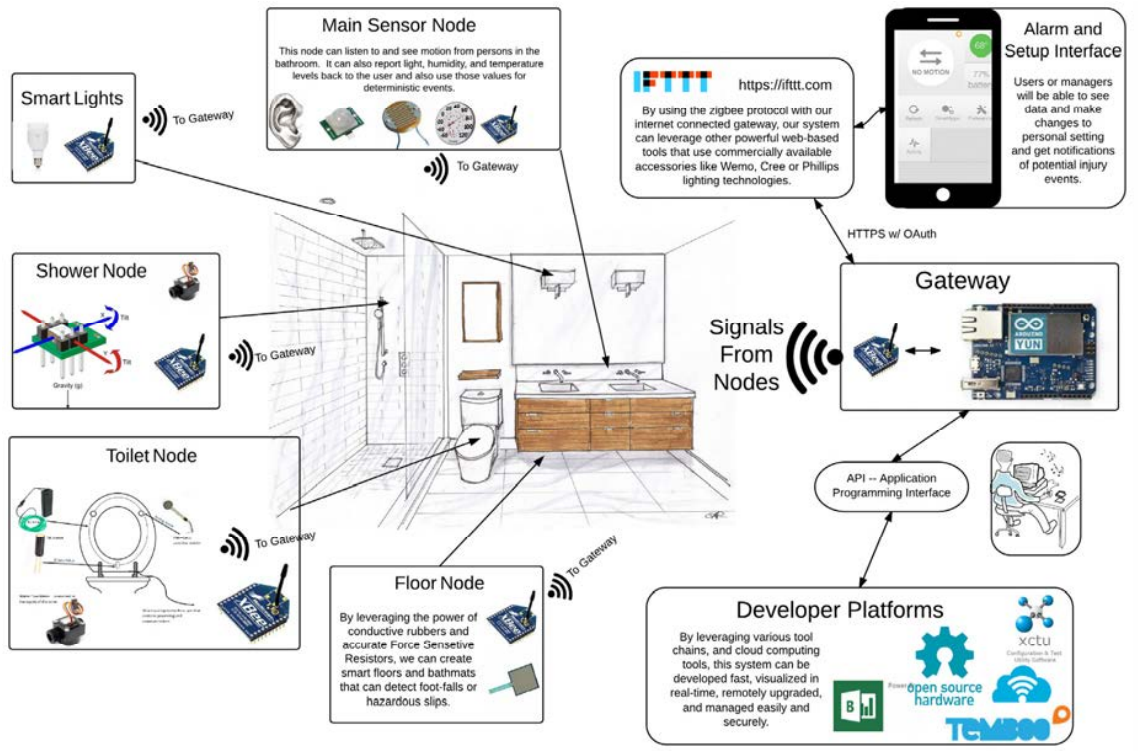
\includegraphics[scale=0.35]{img/paperbathroom.png}
  \caption{La soluzione proposta nel paper}
  \label{fig:usecase_manager}
\end{figure}
\newpage
A livello commerciale, la gestione informatizzata di bagni pubblici si è sviluppata notevolmente negli ultimi anni, grazie sopratutto alla maggiore diffusione ed economicità dell'IoT nel mondo.\\
In linea generale, i prodotti commerciali disponibili possono suddividere in due macro-categorie:
\begin{itemize}
	\item \textit{Sistemi di reportistica}: sono soluzioni che offrono un servizio di reportistica a partecipazione utente, fornendo applicazioni e infrastrutture dal quale è possibile segnalare eventuali problemi riscontrati nell'utilizzo dei servizi pubblici.\\
	Alcuni esempi di prodotti commerciali di questa categoria sono \textit{txt2clean}\cite{txt2clean},\\\textit{restroomalert} \cite{restroomalert} e \textit{Restroom-Management-System}\cite{restroom-management-system}; per fornire un pacchetto più completo, in alcuni prodotti vengono integrate anche alcune funzionalità HR per la gestione del personale.\\
Queste soluzioni sono senza dubbio economiche, ma piuttosto inefficienti: gli addetti alla manutenzione si dovranno affidare a dei semplici feedback per gestire le emergenze, col rischio di incappare in falsi positivi.\\
Inoltre, in questo modo non c'è alcuna prevenzione: le problematiche vengono risolte soltanto dopo la segnalazione (e relativa insoddisfazione) degli utenti.\\
Si tenga presente, infine, che \textit{Smart Public Restroom} prevede già un sistema di reportistica integrato nell'applicazione \textit{Consumer} PWA.
	\item \textit{Sistemi di monitoraggio}: sono prodotti che offrono un monitoraggio completo del servizio igienico grazie all'adozione di sistema composto da un'insieme di sensori appositamente posizionati.\\
	Particolarmente affine si può considerare \textit{Onvation}\cite{onvation}, che sfrutta dispenser smart proprietari di aziende come\textit{Purell} e \textit{Scott} per costruire un sistema smart di monitoraggio e controllo.\\
	Come in \textit{Smart Public Restrooms}, i dati raccolti possono essere aggregati e analizzati grazie ad apposite applicazioni gestionali analoghe a \textit{Manager}; ciò che manca nell'offerta di \textit{Onvation} è un sistema di raccolta feedback degli utenti, che consentirebbe di estrapolare informazioni non direttamente percepibili da sensori.
\end{itemize}
A seguito di questa breve analisi, riteniamo di poter associare \textit{Smart Public Restrooms} a entrambe le categorie di prodotti. 
%----------------------------------------------------------------------------------------
%	ANALISI DEI REQUISITI
%----------------------------------------------------------------------------------------

\section{Analisi dei requisiti}
\subsection{Requisiti}

È necessario realizzare un sistema di gestione per bagni pubblici che consenta a un utente amministrativo, da remoto, di visionare lo stato generale di un impianto.\\
Nel dettaglio ci si aspetta che un utente possa, dato uno specifico impianto, visualizzare in tempo reale:
\begin{itemize}
\item Indicazioni sulla quantità di sapone per le mani rimasto in ogni dispenser, indicato in centesimi.
\item Indicazioni sul tasso di riempimento di ogni pattumiera presente, indicata in centesimi.
\item Indicazioni sullo stato aperto/chiuso di ogni singola cella dell'impianto.
\item Indicazioni sullo stato disponibile/terminata di ogni dispenser di carta igienica presente nelle celle dell'impianto.
\item Indicazioni sullo stato funzionante/non funzionante delle luci di cortesia di ogni cella.
\item Indicazioni sul tasso di umidità di ogni cella dell'impianto.
\item Indicazioni su eventuale presenza di fumo.
\end{itemize}
Le informazioni sopra riportate dovranno essere visionabili attraverso un apposita app chiamata \textit{manager}, che fungerà da supporto gestionale dei bagni pubblici installati.\\
A fronte di un semplice autenticazione tramite utente/password, infatti, l'app dovrà consentire di: 
\begin{itemize}
\item Aggiungere nuovi impianti al sistema.
\item Visualizzare e, all'occorrenza, modificare alcune informazioni di carattere generale sui bagni pubblici installati, come ad esempio indirizzo, coordinate GPS e azienda di manutenzione assegnata.
\item Aggiungere nuovi utenti di amministrazione.
\item Visualizzare eventuali report utente sullo stato del sistema dell'app \textit{consumer}.
\end{itemize}
Si dovrà anche fornire un apposita app (chiamata \textit{consumer}) a supporto di tutti i cittadini e turisti che si vogliono recare in un ambiente pubblico in un certo momento della giornata.\\
L'app dovrà mostrare a schermo la locazione di ogni bagno pubblico (tramite \textit{markers} o simile) disponibile e, all'occorrenza, riportare lo stato degli stessi: qualora un bagno pubblico non sia agibile per qualche motivo, tale informazione dovrà essere opportunamente riportata.\\
Nel dettaglio, l'app \textit{consumer} dovrà consentire di:
\begin{itemize}
\item Visualizzare una \textit{gmap} (centrata sulla locazione corrente) con indicati i bagni pubblici disponibili del sistema.\\Ogni bagno, se selezionato, dovrà mostrare informazioni utili al cittadino circa il loro stato corrente.
\item Riportare direttamente dall'app di eventuali problemi dell'applicazione/dei bagni pubblici riscontrati.
\end{itemize}
\newpage
\subsection{Analisi dei requisiti}
\subsubsection{Glossario}

\begin{center}
    \begin{tabular}{ | l |  p{10cm} |}
    \hline
    \textbf{Name} & \textbf{Definition} \\ \hline
    Impianto & Struttura rappresentante un bagno pubblico, contenente una serie di celle individuali. Ogni impianto è comprensivo di lavabi, dispenser di sapone e pattumiere. \\ \hline
    Cella & Struttura rappresentante una singola unità per servizi igienici comprensiva di gabinetto, carta igienica e luce di cortesia. \\ \hline
    `Manager` web App & Applicazione di amministrazione impianti utilizzata per gestire l'insieme dei bagni pubblici registrati nel network.\\ \hline
    `Consumer` web App & App di supporto al cittadino per individuare il più vicino bagno pubblico e visionare il suo stato corrente.\\ \hline
    gmap & Mappa geolocalizzata 2D fornita gratuitamente da \textit{Google} e molto conosciuta tra gli utenti.\\ \hline
    marker & Marcatore 2D posizionato in coordinate precise della gmap per segnalare la presenza di un punto di interesse.\\ \hline
    Utente amministrativo & Utente adibito a compiti di amministrazione e gestione dei bagni pubblici registrati nella rete, attraverso la web app \textit{manager}.\\ \hline
    Utente consumer & Utente della web app \textit{consumer}. \\ \hline
    \end{tabular}
\end{center}	
\newpage
\subsubsection{Casi d'uso}

\begin{figure}[h!]
  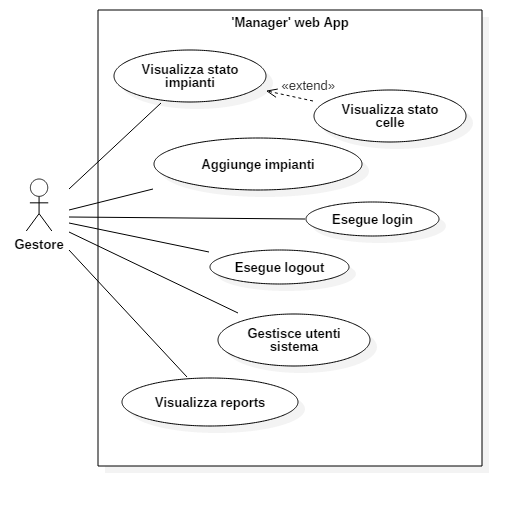
\includegraphics[scale=0.7]{img/usecase_manager.png}
  \caption{Casi d'uso per l'app `manager`}
  \label{fig:usecase_manager}
\end{figure}
\begin{figure}[h!]
  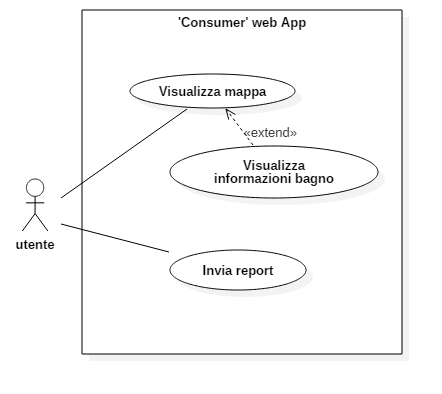
\includegraphics[scale=0.7]{img/usecase_consumer.png}
  \caption{Casi d'uso per l'app `consumer`}
  \label{fig:usecase_consumer}
\end{figure}
\newpage
\phantom{}
\newpage
\subsubsection{Requisiti funzionali}
\begin{enumerate}

\item Ogni sessione di utilizzo di \textit{manager} richiederà un autenticazione nella forma login/password.
\item Ogni impianto dovrà rendere disponibili i seguenti dati:
\begin{itemize}
\item Sapone residuo di ogni dispenser, espresso in centesimi.
\item Spazio residuo (tasso di riempimento) di ogni pattumiera, espresso in centesimi.
\item Eventuale presenza di fumo.
\end{itemize}
Per ogni cella saranno richiesti i seguenti dati:
\begin{itemize}
\item Segnalazione esaurimento carta igienica.
\item Stato di apertura della porta di accesso.
\item Tasso di umidità.
\item Segnalazione guasto luce di cortesia.
\end{itemize}
\item Gli utenti di \textit{manager} dovranno essere in grado di visualizzare i dati inviati dai sensori in tempo reale.
\item Dovrà essere possibile aggiungere nuovi impianti al sistema in qualsiasi momento.
\item Ogni impianto dovrà essere corredato dai seguenti dati:
\begin{itemize}
\item Indirizzo
\item Coordinate GPS
\item Azienda appaltratrice di manutenzione.
\end{itemize}
\item Ogni utente amministrativo di \textit{manager} dovrà essere in grado di creare nuovi utenti di amministrazione.
\item Ogni utente amministrativo di \textit{manager} dovrà essere in grado di visualizzare i reports utente sullo stato degli impianti o dell'app \textit{consumer}.
\item L'app \textit{consumer} dovrà adeguatamente funzionare su dispositivi mobili come smartphone e tablet con Android 8+ o iOS 11+.
\item L'app \textit{consumer}, all'avvio della gmap, dovrà centrarsi sulla posizione geolocalizzata del dispositivo.
\item La gmap di \textit{consumer} dovrà mostrare tutti gli impianti registrati nel sistema con appositi \textit{marker}.
\begin{enumerate}
\item Ogni impianto selezionato servirà per mostrare all'utente il suo stato corrente, con particolare attenzione circa la sua disponibilità.
\end{enumerate}
\item Ogni utente di \textit{consumer} potrà rilasciare, attraverso l'app, una segnalazione sullo stato dei servizi riscontrati.
\item \textit{consumer} dovrà essere nativamente installabile sul dispositivo dell'utente.
\end{enumerate}
\subsubsection{Requisiti non funzionali}
\begin{itemize}
\item \textbf{Dinamicità:} Il sistema dovrà consentire l’aggiunta e la rimozione di impianti sul territorio dinamicamente senza causare interruzioni generali del servizio.\\ Il sistema, pertanto, dovrà risultare adattabile ai cambiamenti della topologia di rete di cui è composto.
\item \textbf{Scalabilità:} Il sistema dovrà essere adattabile alla mole di informazioni inviata dagli impianti ed essere sufficientemente reattivo nei confronti delle richieste degli utenti, che aumenteranno gradualmente mano a mano che il sistema verrà adottato su tutto il territorio.\\
Verosimilmente, adottando il sistema su scala nazionale per i soli bagni pubblici, il numero di impianti da gestire si attesterà su qualche centinaio.\\
Anche considerando la partecipazione di bagni pubblici di natura privata (si pensi ai bagni degli autogrill), il numero totale di impianti non dovrebbe superare il migliaio di unità.\\ 
Il numero di utenti di amministrazione, considerati i punti sopra, dovrebbe rimanere pressoché trascurabile.\\
Gli utenti \textit{consumer}, d'altro canto, potranno raggiungere numeri considerevoli: particolare attenzione alla scalabilità dovrà essere riposta nello sviluppo dell'app per dispositivi mobili.
\item \textbf{Prestazioni:} Il sistema dovrà essere in grado di rispondere a tutte le richieste a cui andrà incontro con prestazioni ottimali, minimizzando il tempo di attesa di ogni azione intrapresa dagli utenti.\\
Dal punto di vista puramente applicativo, l'applicazione dovrà essere fluida nei caricamenti e nelle transizioni: ciò sarà possibile attraverso l'utilizzo di tecnologie all'avanguardia e restringendo il bacino di utenza dell'applicazione ai soli dispositivi più aggiornati.\\
Considerando la mole di dati coinvolta (e la loro non-criticità), si potrebbe considerare accettabile un aggiornamento dei valori di ogni impianto con intervalli di 10 secondi.
\item \textbf{Robustezza:} Il sistema dovrà offrire una buona tolleranza a tutti i guasti che si potranno presentare quotidianamente: errori di rete, anomalie delle letture dei sensori,  malfunzionamenti hardware ecc..\\ 
Gli eventuali malfunzionamenti riscontrati, infatti, non dovranno compromettere l'intero funzionamento del sistema ma soltanto le risorse direttamente collegate ad esso.\\ 
Eventuali fallimenti hardware (sia dei sensori che dei microcontrollori presenti) dovranno essere risolvibili sostituendo i singoli componenti difettosi, evitando così costose riconfigurazioni del sistema.\\
Qualora il server di sistema diventasse irraggiungibile, gli utenti \textit{consumer} dovranno comunque poter utilizzare l'app offline.

\item \textbf{Sicurezza:} Essendo le applicazioni esposte pubblicamente sulla rete, è importante che esse seguano i più elevati standard di sicurezza.\\
Tutte le applicazioni dovranno essere essere servite su HTTPS e protette da eventuali tentativi di attacco XSS da parte degli utenti.\\
Tutti gli accessi all'applicazione \textit{manager} (e, di conseguenza, al Database) necessiteranno di essere autenticati per limitare la superficie d'attacco di eventuali attori.\\
L'app consumer, venendo installata sul dispositivo degli utenti e possibilmente di milioni di persone, dovrà seguire i più elevati standard di sicurezza per evitare \textit{man-in-the-middle attacks} e qualsiasi uso non autorizzato dei servizi sopra descritti.

\item \textbf{Interoperabilità:} il sistema dovrà essere progettato per favorire il più possibile l'adozione di standard riconosciuti e, possibilmente, open-source.\\
In tal modo sarà possibile adattare il sistema a molteplici scenari e integrarlo con strumenti di terze parti, qualora lo si ritenga necessario.
\end{itemize}
%----------------------------------------------------------------------------------------
%	PROGETTAZIONE
%----------------------------------------------------------------------------------------
\newpage
\section{Progettazione}
\subsection{Architettura del sistema}

Una breve analisi dei requisiti in un ottica progettuale ci porta a una suddivisione del sistema in tre parti logiche ben distinte: 
\begin{itemize}
	\item Una parte \textit{locale}, installata fisicamente in ogni impianto della rete, dedita alla raccolta di dati tramite sensori e al loro periodico invio.
	\\ Tutta l'insieme della componentistica hardware (e le relative problematiche) del progetto sarà concentrata in questa macro-area.
	\item Una parte \textit{applicativa}, dedita all'analisi dei dati raccolti, da parte di personale amministrativo e utenti \textit{consumer}.
	\item Una parte \textit{centrale}, costituita da un server (o, possibilmente, un insieme di server) dedita alla ricezione e archiviazione dei dati inviati dalle parti \textit{locali} del network.\\
	Questa entità si occuperà anche di distribuire le applicazioni (\textit{manager} e \textit{consumer}) agli utenti del sistema.
\end{itemize}

Una tale suddivisione del sistema consente di soddisfare pienamente i requisiti presentati nel capitolo precedente: la presenza di un \textit{middleware} (cioè il server)  tra le parti applicative e le parti locali consente di aumentare considerevolmente la sicurezza e la scalabilità dell'intero network.\\\\
La comunicazione tra la parte \textit{centrale} e parti \textit{applicative} e \textit{locali} avverrà tramite interfaccia RESTful, garantendo così i seguenti vantaggi:
\begin{itemize}
	\item \textit{Stateless}: non mantenendo su server alcuna informazione circa il contesto durante la connessione, ogni sessione utente è più sicura, performante e semplice.
	\item Compatibilità: essendo riconosciuto come standard \textit{de facto} nelle comunicazioni client-server (in virtù anche dei suoi requisiti meno stringenti rispetto ad altre forme di trasmissione formali come WSDL) è del tutto ragionevole considerare RESTFul un interfaccia applicabile in qualsiasi contesto di rete moderno.
	\item Affidabilità: una trasmissione RESTful JSON è composta sostanzialmente da una connessione HTTP tramite TCP/IP con un formato dati a bassissimo \textit{overhead}.\\
	Pertanto, ogni connessione si concluderà con un singolo invio di dati:  ciò rende questa forma di comunicazione appetibile in contesti in cui non è possibile assicurare una connessione di rete stabile.
\end{itemize}
Viene riportato un diagramma dell'architettura logica della progettazione appena descritta:
\begin{figure}[h!]
\centering
  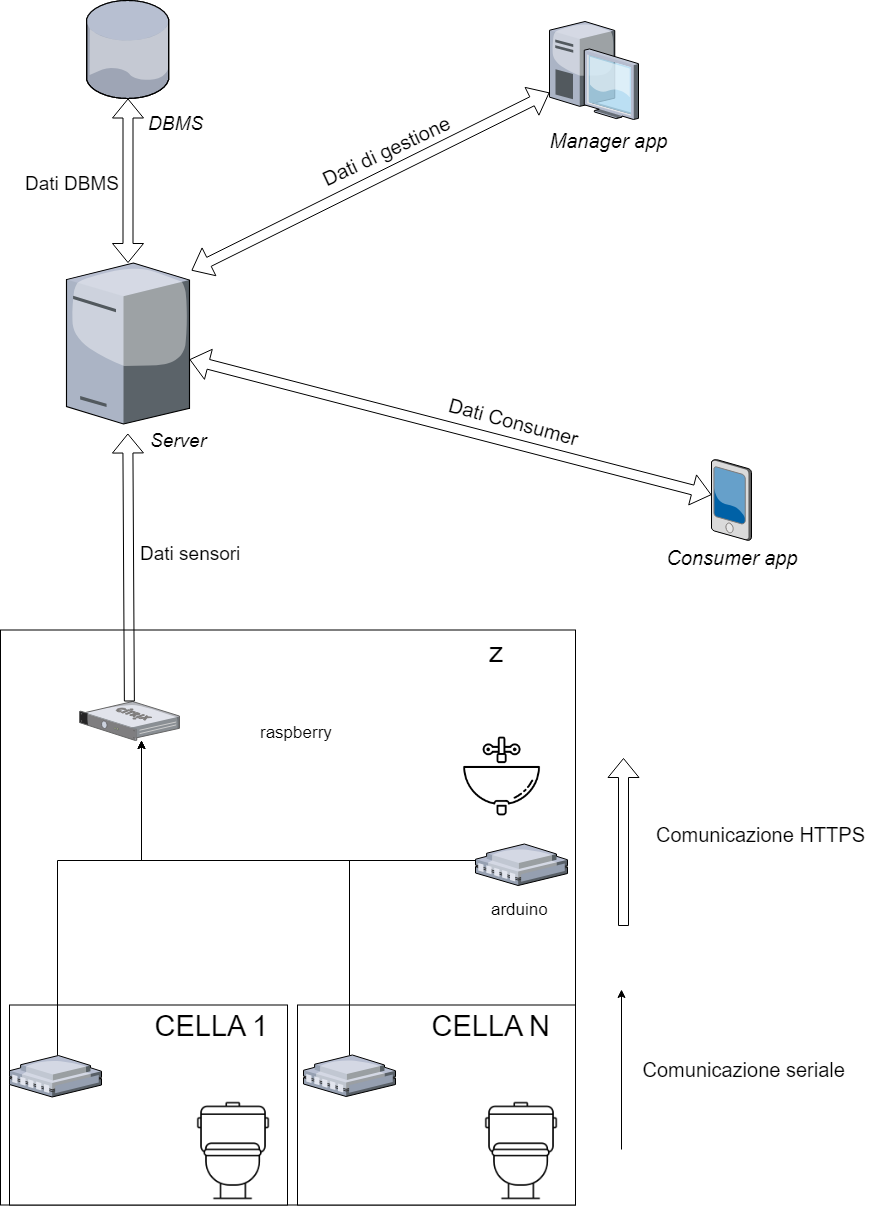
\includegraphics[scale=0.33]{img/architettura_logica-report.png}
  \caption{Architettura logica del sistema}
\end{figure}
\subsection{Progettazione parte locale}
La progettazione della parte locale prevede il sistema di produzione dei dati grezzi, dalla loro generazione fino all'invio al server.
Sulla base dei requisiti non funzionali, il progetto della parte locale deve tenere in considerazione due fattori principali:
\begin{itemize}
	\item \textbf{Versatilità del sistema.}
	Il sistema deve essere progettato in modo tale da poter essere riutilizzabile e adattabile a qualsiasi tipo e forma di locale in esercizio. 
	\item \textbf{Costo di realizzazione dell'impianto.}
	Il costo dell'impianto deve essere il più contenuto possibile.
\end{itemize}  
\subsubsection{Progettazione hardware}
La scelta dell'hardware incide molto sui fattori di versatilità e costi. Occorre quindi pensare a come ottenere i dati necessari in modo economico e affidabile. Per la progettazione dell'hardware si procede con la tecnica bottom-up, si illustrano prima i dispositivi scelti e il pensiero dietro di essi in modo da ricavare i dati grezzi. Poi si assemblano le varie componenti insieme per ottenere una struttura più complessa e di rilievo a livello di business. Di seguito i vari concept.
\paragraph{Sensori}
I sensori sfruttati sono i seguenti
\begin{itemize}
\item Fotoresistori
\item Emettitori laser
\item DHT21 (Rilevamento temperatura e umidità)
\item Sensori ultrasuoni
\item Sensori di forza
\item Sensori di fumo
\end{itemize}
\subparagraph*{Porta chiusa e disponibilità carta igienica - Coppia emettitore laser e fotoresistore}
L'\textit{emettitore laser} è un dispositivo elettronico rappresentabile da un diodo che emette un fascio di luce concentrato verso una direzione.
Il \textit{fotoresistore} è un dispositivo elettronico rappresentabile da una resistore (o resistenza variabile) che regola la sua resistenza in base alla luce che riceve sulla sua componente fotosensibile; più è la luce che riceve, minore è la resistenza.
Le due componenti le si possono utilizzare per concentrare la luce in un unico punto del fotoresistore trasformando la coppia di sensori in un interruttore; si considera il l'interruttore chiuso quando il fotoresistore mostra una resistenza al di sotto di una certa soglia.
E' possibile sfruttare questa coppia per sapere se una porta è chiusa o se la carta igienica è disponibile.
\begin{figure}[h!]
\centering
	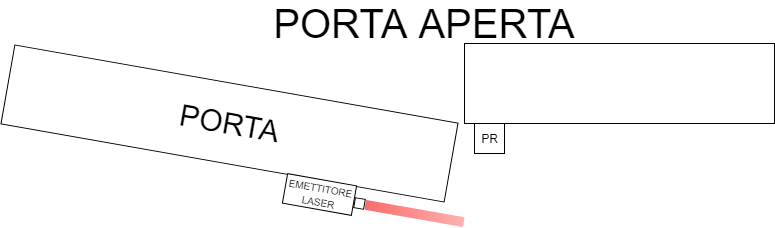
\includegraphics[scale=0.45]{img/parteLocale/PortaAperta.png} 
    \caption{Interruttore aperto}
\end{figure}

\begin{figure}[h!]
\centering
	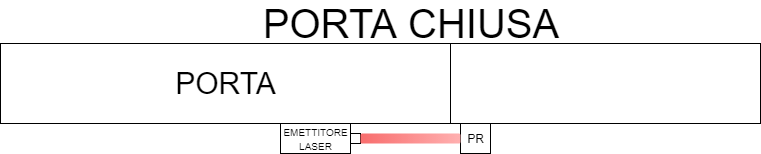
\includegraphics[scale=0.45]{img/parteLocale/PortaChiusa.png} 
    \caption{Interruttore aperto}
\end{figure}
Una porta si definisce chiusa quando la luce del laser è concentrata sul fotoresistore, aperta altrimenti.


\newpage
La carta igienica si definisce esaurita quando la luce del laser è concentrata sul fotoresistore,disponibile altrimenti.
\begin{figure}[h!]
\centering
	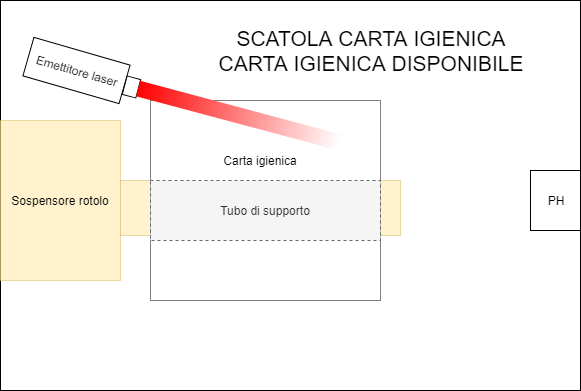
\includegraphics[scale=0.55]{img/parteLocale/CartaIgienicaDisponibile.png}  
    \caption{Interruttore aperto}
\end{figure}

 
 \begin{figure}[h!]
\centering
	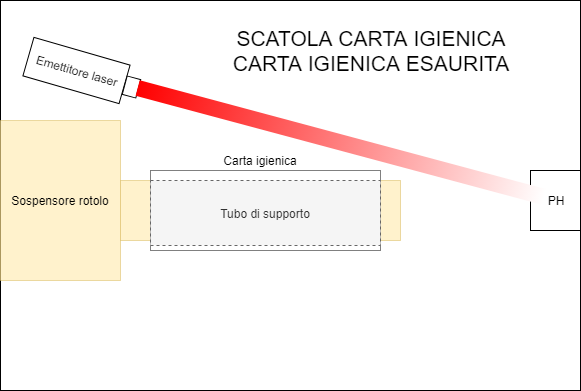
\includegraphics[scale=0.55]{img/parteLocale/CartaIgienicaEsaurita.png}  
    \caption{Interruttore chiuso}
\end{figure}
Poichè il cartone di supporto del rotolo di carta igienica tende alla deformazione, è possibile che il laser non tocchi il fotoresistore anche se la carta igienica è finita.
 \begin{figure}[h!]
\centering
	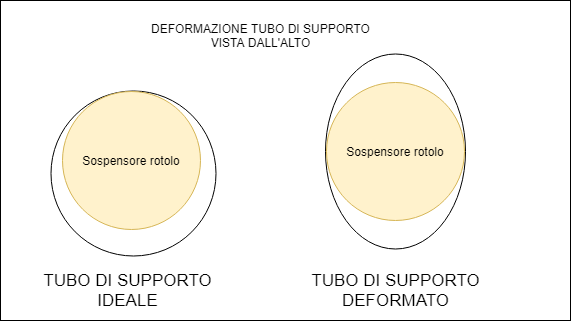
\includegraphics[scale=0.55]{img/parteLocale/DeformazioneTubo.png}  
    \caption{Deformazione del tubo di supporto alla carta igienica}
\end{figure}
 \begin{figure}[h!]
\centering
	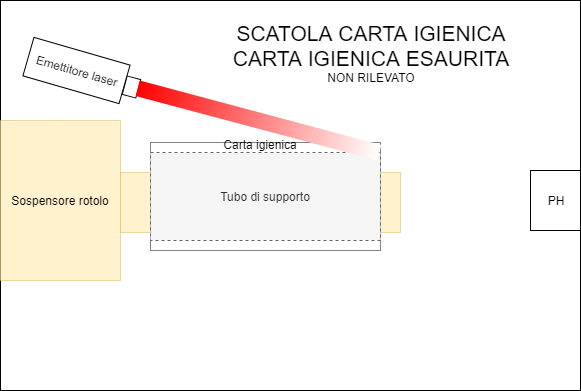
\includegraphics[scale=0.55]{img/parteLocale/ProblemaDeformazione.png}  
    \caption{Interruttore erroneamente aperto}
\end{figure}
Per ovviare al problema è sufficiente aggiungere un altro emettitore laser che puntano allo stesso fotoresistore da un punto differente rispetto al primo.
 \begin{figure}[h!]
\centering
	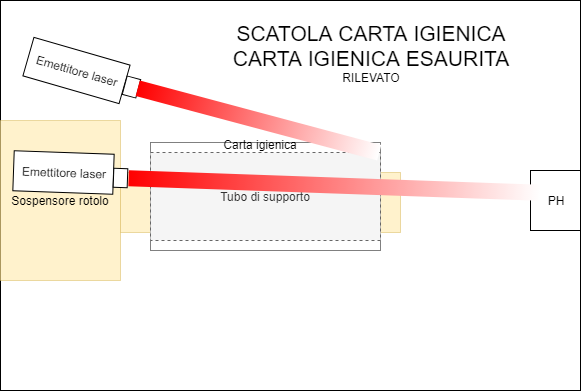
\includegraphics[scale=0.55]{img/parteLocale/SoluzioneDeformazione.png}  
    \caption{Interruttore chiuso}
\end{figure}
\subparagraph{Guasto luce - fotoresistore}
Un singolo fotoresistore è in grado di avvertirci se c'è un guasto alla luce

\subparagraph{Rilevamento umidità celle - DHT21}
Il DigitalHumidityTemperature (DHT) è un sensore digitale complesso che permette di rilevare l'umidità e la temperatura dell'ambiente che lo circonda. Non richiede installazioni complesse, è sufficiente installarlo a mezzo metro dal soffitto per un rilevamento ideale.
\subparagraph{Rilevamento spazzatura - Sensore a ultrasuoni}
Il sensore a ultrasuoni è un sensore digitale complesso che permette di calcolare la distanza tra esso e l'oggetto che ha di fronte. Il sensore emette un segnale a ultrasuoni e stima la distanza aspettando e calcolando il tempo di ritorno di quel segnale.
L'idea è di piazzare il sensore sotto il coperchio del bidone della spazzatura e puntarlo verso la base del bidone. Man mano che il bidone si riempie il sensore dovrebbe stimare distanze sempre minori fino a raggiungere la distanza minima e avvertire quindi che il bidone è pieno.
\subparagraph{Rilevamento presenza sapone - Sensore di forza}
Il sensore di forza è un sensore di tipo analogico rappresentabile da un resistore che permette di rilevare il peso degli oggetti posizionati su di esso. L'idea quindi è quella di piazzare il sensore sotto il contenitore del sapone liquido, stimando la quantità di sapone rimasto nel contenitore in base al suo peso. Se il contenitore è pieno si avrà più peso sul sensore. 
\subparagraph{Rilevatore di fumo}
Il rilevatore di fumo è un sensore analogico complesso rappresentabile da un resistore che varia la sua resistenza interna in base alla presenza di gas nell'atmosfera a se circostante. Non richiede installazioni complesse se non il montaggio su soffitto per rilevare la presenza di gas leggeri come il monossido di carbonio o il fumo in generale.
\paragraph{Arduino-like}
Poiché il personale non ha conoscenze approfondite in ingegneria elettronica, per risparmiare tempo e contenere i costi di progettazione di un possibile circuito elettronico, si è sfruttato l'utilizzo dei microcontrollori programmabili come l'Arduino..
Dall'analisi s'illustra che è necessario installare un dispositivo Arduino-like per la gestione dei dispositivi in ogni cella e un unico dipositivo Arduino-like per la gestione dei dispositivi ai lavabi.\\
 \begin{figure}[h!]
\centering
	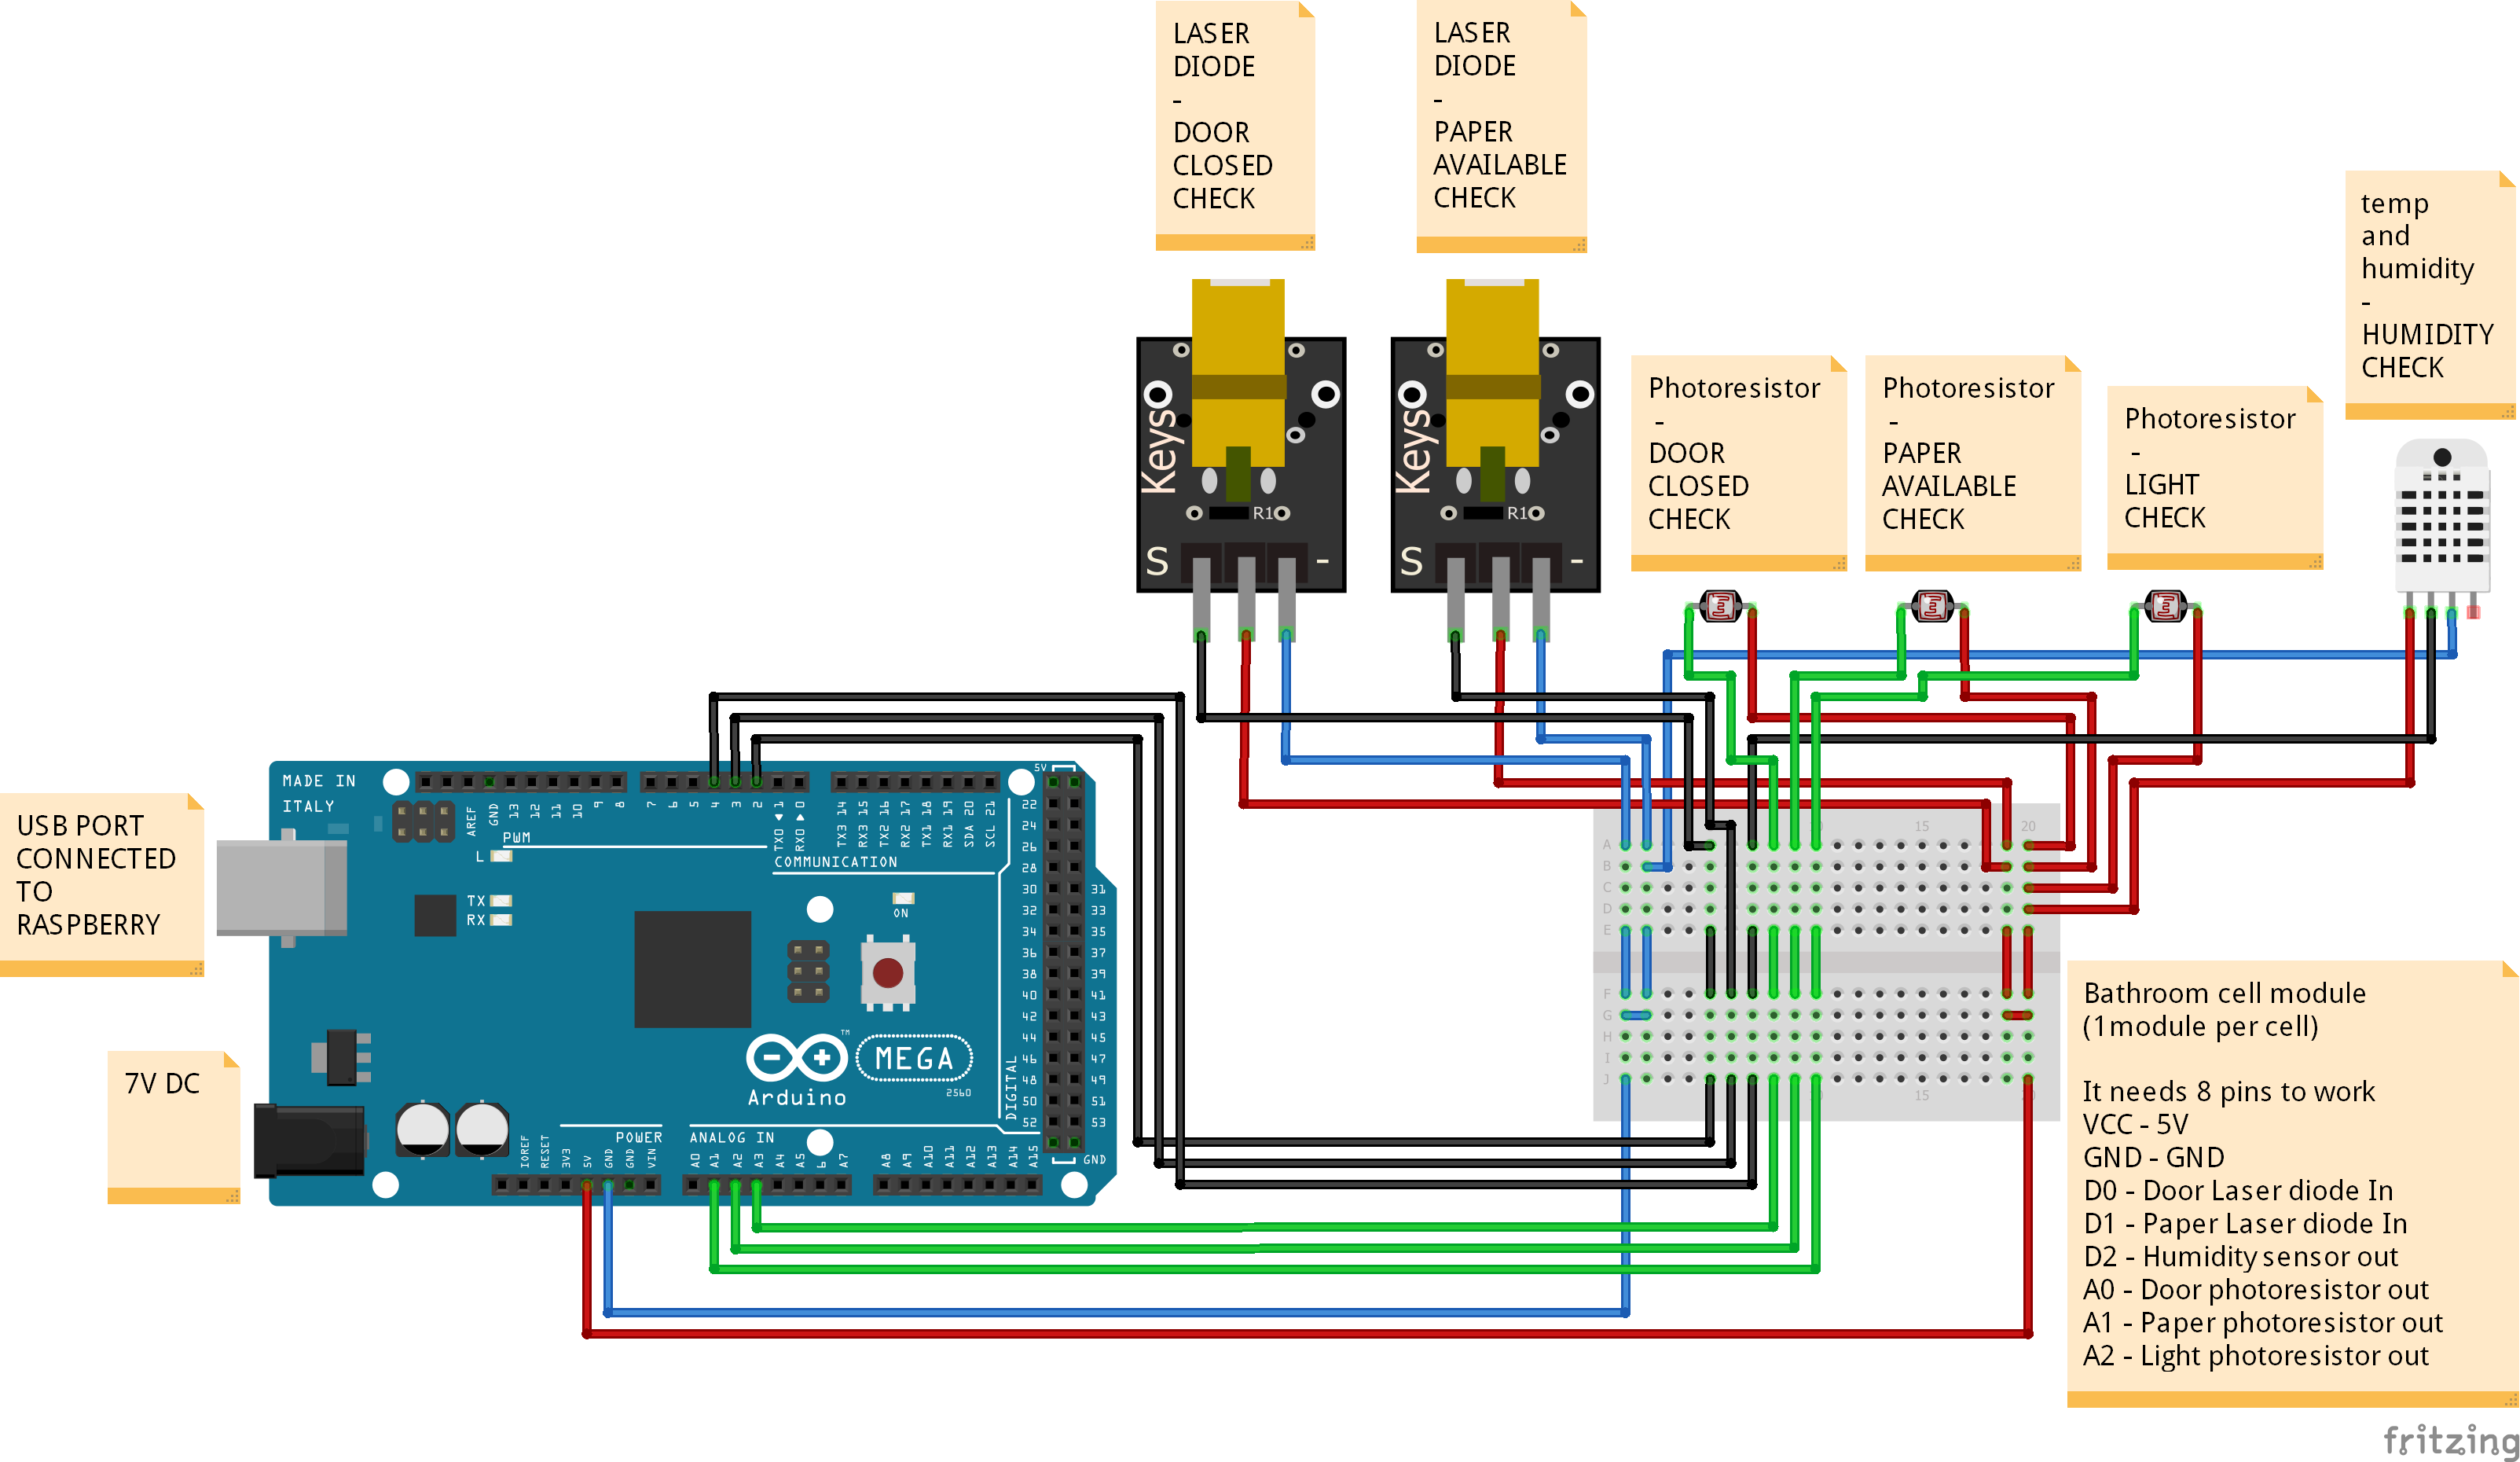
\includegraphics[scale=0.45]{img/RestroomCell_bb.png}  
    \caption{Circuito cella}
\end{figure}
 \begin{figure}[h!]
\centering
	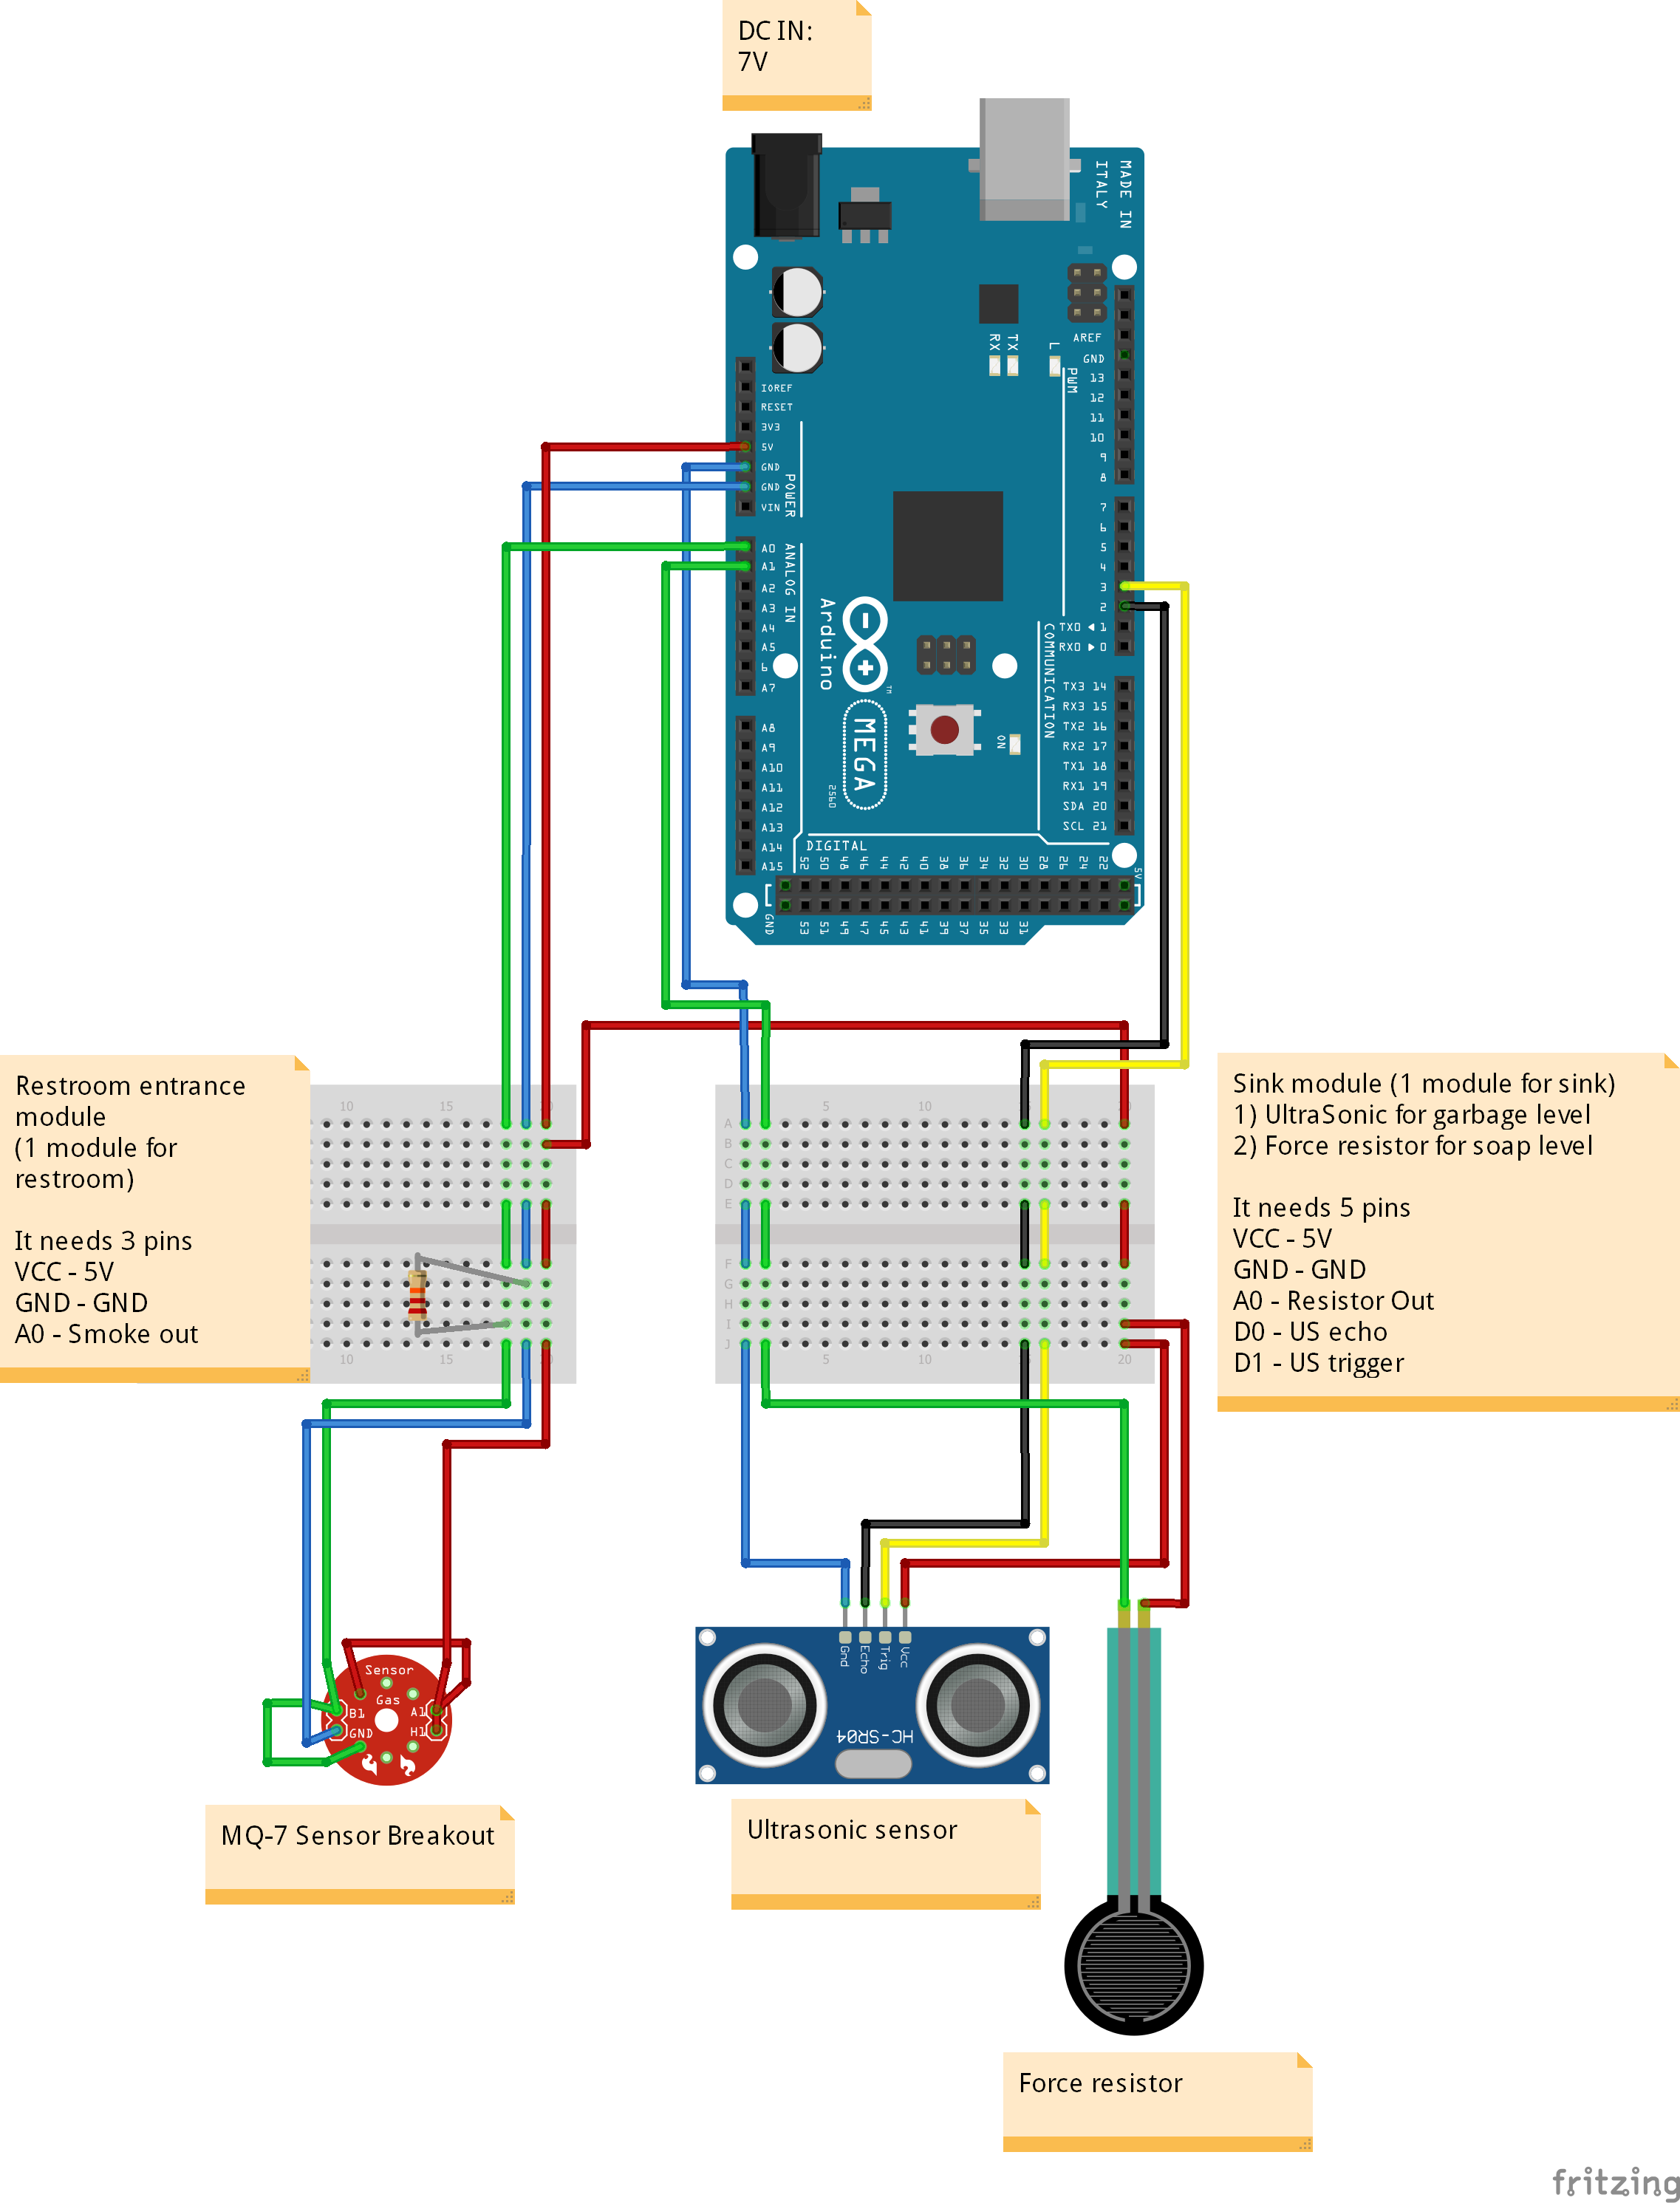
\includegraphics[scale=0.45]{img/RestroomEntry_bb.png}  
    \caption{Circuito lavabo}
\end{figure}
\\Da come si evince dalle immagini sopra riportate, l'Arduino è alimentabile da porta usb ma per una maggiore stabilità verranno sfruttati degli alimentatori da 220Vin-7VOut.
Ogni Arduino è in grado di alimentare tutti i sensori ad esso collegati, di leggere il loro stato (come per il dht) o cambiare il loro stato (come per l'emettitore laser)
L'Arduino tuttavia ha grosse limitazioni per quanto riguarda la memoria disponibile e la potenza computazionale; motivo per cui tutto il carico di lavoro che riguarda la manipolazione dei dati grezzi e il delivering dei dati strutturati viene spostato su un dispositivo più prestante e adatto al compito: il Raspberry.
\paragraph{Raspberry}
Il Raspberry è un dispositivo IOT sufficientemente potente da poter essere sfruttato come aggregatore di dati per l'intero sistema locale. Tramite le porte usb ha il compito di connettersi e comunicare con i dispositivi Arduino raccogliendo quindi i dati grezzi.
Una volta manipolati i dati grezzi, il Raspberry ha il compito di spedire i dati elaborati al server dove infine verranno salvati.
\subsubsection{Progettazione software arduino}
L'Arduino è il dispositivo responsabile alla comunicazione dei sensori con il Raspberry.
In base all'analisi dei requisiti si può dedurre che l'Arduino ha bisogno di essere configurato per due tipi di ambienti:
\begin{itemize}
\item L'ambiente della cella
\item L'ambiente dei lavabi
\end{itemize}
L'Arduino ha lo svantaggio di avere poca memoria interna e un'architettura non in grado di gestire il multithreading. La complessità della struttura del programma che verrà caricato sul dispositivo potrebbe compromettere l'affidabilità dell'intero sistema hardware; questo problema ci obbliga a progettare un software molto leggero e statico.
Di seguito viene riportato quindi un UML di progetto compatibile con due software molto simili tra loro affinché l'Arduino possa essere installato in entrambi i tipi di ambiente. 
\begin{figure}[h!]
\centering
	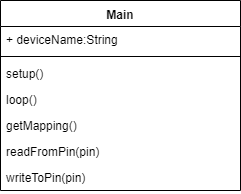
\includegraphics[scale=0.55]{img/parteLocale/SoftwareArduino.png}  
    \caption{Classe principale del software Arduino}
\end{figure}
\subsubsection{Progettazione software raspberry}
Il Raspberry è un computer economico con architettura Arm a basso consumo energetico; in questo progetto il suo compito è quello di ricevere i dati grezzi dall'Arduino, di manipolarli e poi spedire i dati elaborati al server centrale.
\paragraph{Ambiente di sviluppo}
Il Raspberry supporta un qualsiasi sistema operativo Arm ma è Raspbian il sistema operativo scelto poiché il più supportato dalla community nonché il più ottimizzato tra tutti. Verranno usati principalmente tre paradigmi di programmazione: 
\begin{itemize}
\item OOP
\item Programmazione funzionale 
\item Programmazione reattiva. 
\end{itemize}
\paragraph{Concetto del software lato raspberry}
Si è progettato il software del raspberry in modo che i concetti di business coincidano il più possibile con le problematiche tecniche da risolvere.
Il software può essere diviso concettualmente in due parti:
\begin{itemize}
\item Sensori
\item Manager
\end{itemize}
\subparagraph{Sensori virtuali}
\begin{figure}[h!]
\centering
	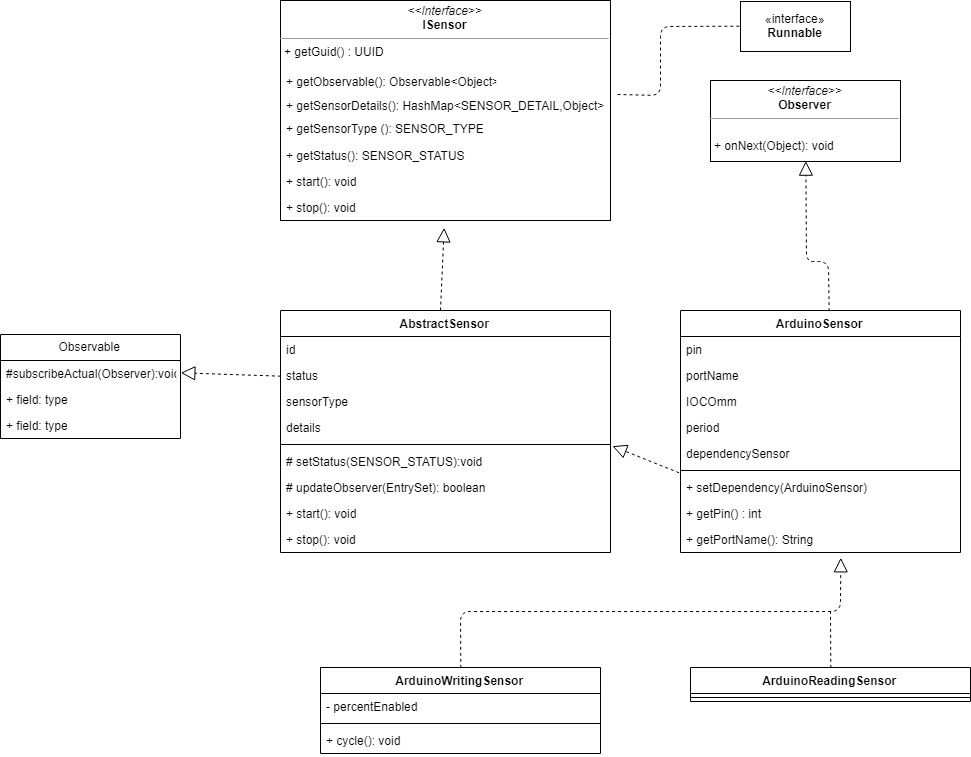
\includegraphics[scale=0.35]{img/parteLocale/SoftwareSensorsRaspberry.png}  
    \caption{Classe principale del software Arduino}
\end{figure}
I sensori virtuali sono componenti software gestiti da thread indipendenti l'uno dall'altro che hanno il compito di recuperare i dati dai sensori fisici e spedirli al Manager.
E' possibile che un sensore sia dipendente da altri sensori per il corretto funzionamento; in questo caso il sensore dovrà abilitare il sensore padre prima di avviare la lettura.
\begin{figure}[h!]
\centering
	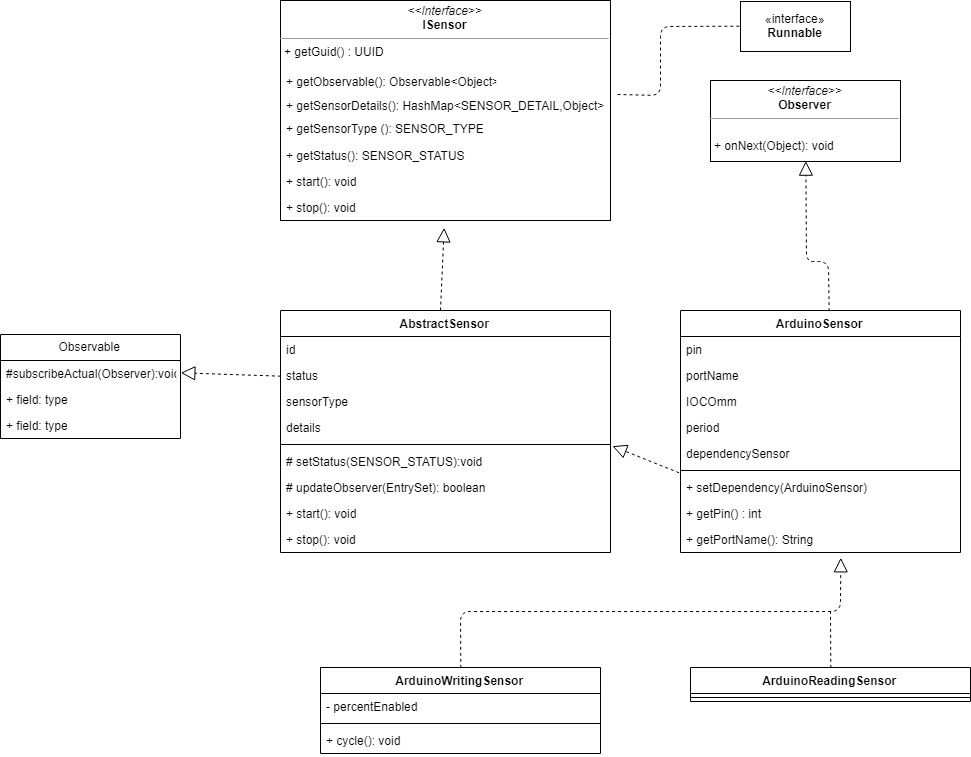
\includegraphics[scale=0.43]{img/parteLocale/SoftwareSensorsRaspberry.png}  
    \caption{Classe principale del software Arduino}
\end{figure}
\newpage
\subparagraph{Manager}
[UML RELATIVO ALL'IManager e sue implementazioni]
Il manager è un componente software che ha il compito di eseguire le seguenti funzioni:
\begin{itemize}
\item Connettersi ai vari dispositivi Arduino
\item Inizializzare tutti i sensori virtuali mappandoli con i sensori fisici.
\item Attivare o disattivare la lettura dei sensori virtuali
\item Attendere la ricezione dei dati da parte dei sensori virtuali
\item Aggregare i dati ricevuti in un'unica struttura
\item Inviare i dati strutturati,se necessario con politiche di temporizzazione, al server
\end{itemize}
\subsubsection{Progettazione interazione raspberry arduino}
Come precedentemente scritto, i sensori virtuali dovranno essere gestiti da thread indipendenti l'uno dall'altro ma è stato anche specificato che devono interfacciarsi con l'Arduino, un microcontrollore con risorse computazionali molto basse. La progettazione della parte locale deve quindi prevedere una metodologia efficace affinché l'Arduino possa ricevere un input consistente da ogni thread interessato a interrogarlo e rispondere a questi thread di conseguenza.
\paragraph{Concetto arduino-server like}
L'idea è quella di far interagire il Raspberry con l'Arduino come se l'Arduino fosse un server e il Raspberry il suo client. La comunicazione avverrà tramite la porta seriale quindi si useranno le stringhe per inviare e ricevere messaggi.  
[IMMAGINE INTERAZIONE RASPBERRY-ARDUINO CLIENT-SERVER]
\subparagraph{Arduino as a server}
L'arduino espone un numero definito di metodi. E' possibile accedere a questi metodi tramite una linea di stringa strutturata. L'Arduino si mette in attesa di possibili stringhe di richiesta da parte del Raspberry e accumula le riceventi all'interno del buffer della sua seriale.
Ogni linea di richiesta viene presa dal buffer consumandola per poi effettuare un rapido parsing di conformità. Se la richiesta è valida, l'Arduino elabora la risposta e la manda indietro attraverso la porta seriale sotto forma di messaggio strutturato.
\subparagraph{Raspberry as a Client}
Dal lato raspberry un sensore virtuale, per comunicare col raspberry, deve creare una nuova stringa di richiesta e inserirla in una coda. 
Il manager si occupa quindi di svuotare la coda mandando messaggi di richiesta all'Arduino solo quando quest'ultimo è in grado di ascoltare. Nel frattempo il manager si mette in ricezione di possibili messaggi di risposta dall'Arduino. Ogni messaggio di risposta andrà poi a popolare una coda di ricezione; il manager si occuperà quindi di svuotare la coda smistando i messaggi di risposta ai destinatari corretti.
Questo tipo d'interazione verrà sfruttato principalmente dal manager stesso per recuperare dai vari Arduino le loro mappature; in questo modo il manager potrà inizializzare correttamente i sensori virtuali.
\newpage
\subsection{Progettazione parte applicativa}
Grazie all'analisi dei requisiti effettuata, si è evidenziato come il committente abbia richiesto la creazione di due applicazioni distinte, ognuna con una diversa finalità.\\
Purtroppo, ciò si scontra con la realtà del team di sviluppo incaricato alla produzione di \textit{manager} e \textit{consumer}: le risorse a disposizione sono piuttosto esigue, sia in termini di tempo che di manodopera.\\
Pertanto, come vedremo, verranno adottate strategie atte a ridurre i costi di sviluppo e rientrare, così, nel budget e nei tempi previsti.\\\\
Si tenga presente, inoltre, che data la loro reciproca indipendenza, ogni applicazione verrà analizzata separatamente nelle sottosezioni seguenti.
\subsubsection{Manager}
\paragraph{Ambiente}
I requisiti esposti dal committente riguardo la realizzazione di \textit{manager} non specificano il suo ambiente di utilizzo preferenziale: gli utenti potrebbero lavorare su macchine Windows o Linux indifferentemente.\\
A seguito di questa considerazione, e in relazione al fatto che non sono stati richieste funzionalità native specifiche di un qualche ambiente, si è deciso di realizzare \textit{manager} come \textit{web appplication}.\\
Tuttavia, sviluppare un'applicazione amministrativa per ambienti web  non consente soltanto di renderla pressoché universale, ma garantirà anche i seguenti benefici:
\begin{itemize}
\item Faciliterà la fase di distribuzione, in quanto non necessiterà di installazione locale (gli utenti potranno accedere all'applicazione attraverso un semplice browser web, che si presume già installato di default in tutti i sistemi operativi moderni).
 \item Renderà lo sviluppo della stessa più semplice, perché familiare all'insieme di skill pregresse del team di sviluppo.
\end{itemize}
Per rendere l'esperienza utente il più possibile vicina a una classica \textit{dekstop application} gestionale, \textit{manager} verrà sviluppata come una SPA (\textit{Single Page Application)}.\\\\
La decisione di sviluppare \textit{manager} per ambienti web, tuttavia, ha un costo ben definito in termini di compatibilità: il supporto ad alcune tecnologie per SPA, infatti, non potrà essere garantito  e ciò potrà portare ad escludere alcuni dispositivi particolarmente datati.
\paragraph{Autenticazione}
I requisiti esposti dal committente richiedono esplicitamente che gli utenti di amministrazione che utilizzano \textit{manager} debbano essere autenticati nel sistema, preferibilmente attraverso l'uso di username e password.\\
Data l'assenza di indicazioni in merito, il team di sviluppo si concentrerà solamente sulla realizzazione di autenticazioni con un singolo ruolo immutabile, ovvero quello di ``amministratore''; in altre parole, in questa prima iterazione del software qualsiasi utente connesso avrà pieno accesso a tutte le funzionalità del software.\\\\
Per evitare che ogni funzionalità ``protetta'' del prodotto richieda una forma di autenticazione all'utente, \textit{manager} utilizzerà un \textit{access token} scambiato dal server per ogni accesso successivo.\\
Tale \textit{access token} sarà costituito da una stringa casuale univoca e verrà salvato localmente nel browser utente: a tal scopo, esso verrà utilizzato come chiave di identificazione ad ogni successivo avvio dell'app, se presente.\\\\
È necessario tenere presente, tuttavia, che l'utilizzo di questo metodo di autenticazione non è esente da difetti o possibili rischi:
\begin{itemize}
\item Come qualsiasi altra risorsa locale salvata sul terminale utente, il \textit{loginToken} può essere accidentalmente (o volutamente) cancellato.\\ Purtroppo, questo rischio è particolarmente sentito in ambito web a causa alla relativa facilità con la quale è possibile cancellare la cache locale.
\item L'utilizzo di una chiave di accesso può esporre il sistema a rischi legati alla sicurezza: un terminale compromesso da un utente malintenzionato finirà infatti per esporre pubblicamente la propria chiave di accesso (attualmente, purtroppo, non vi è modo di archiviare in sicurezza le risorse locali di un browser).\\
Ottenuto così un \textit{loginToken} autentico, l'utente malintenzionato potrà effettuare attacchi \textit{masquerade} con la minima probabilità di essere scoperto.
\end{itemize}
Per rafforzare ulteriormente la sicurezza del sistema, inoltre, sarebbe opportuno associare un periodo di validità (ad esempio, 7 giorni) ad ogni \textit{loginToken}.\\
Qualora un utente non abbia effettuato l'accesso per un certo periodo prestabilito, infatti, la sessione sarà da riconvalidare con un nuovo accesso tramite i canali tradizionali.\\\\
Viene quindi presentato un breve diagramma di attività che riassume il funzionamento della login di \textit{manager}:
\begin{figure}[h!]
\centering
  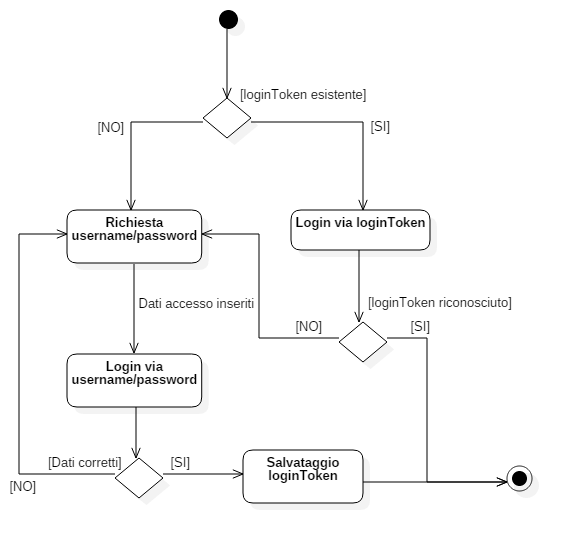
\includegraphics[scale=0.6]{img/activity_manager.png}
  \caption{Login \textit{manager}}
\end{figure}
\paragraph{Design}
Trattandosi di un applicazione di gestione e amministrazione, \textit{manager} non presenterà un'interfaccia ottimizzata per dispositivi mobili: si presume infatti che tutti gli utenti del sistema utilizzeranno il prodotto tramite uno schermo con sufficiente larghezza (ad esempio tramite un PC Fisso).\\Per questo motivo, il design si è incentrato su un interfaccia tipica per dispositivi desktop, come evidenziabile dal mockup seguente: 
\begin{figure}[h!]
\centering
  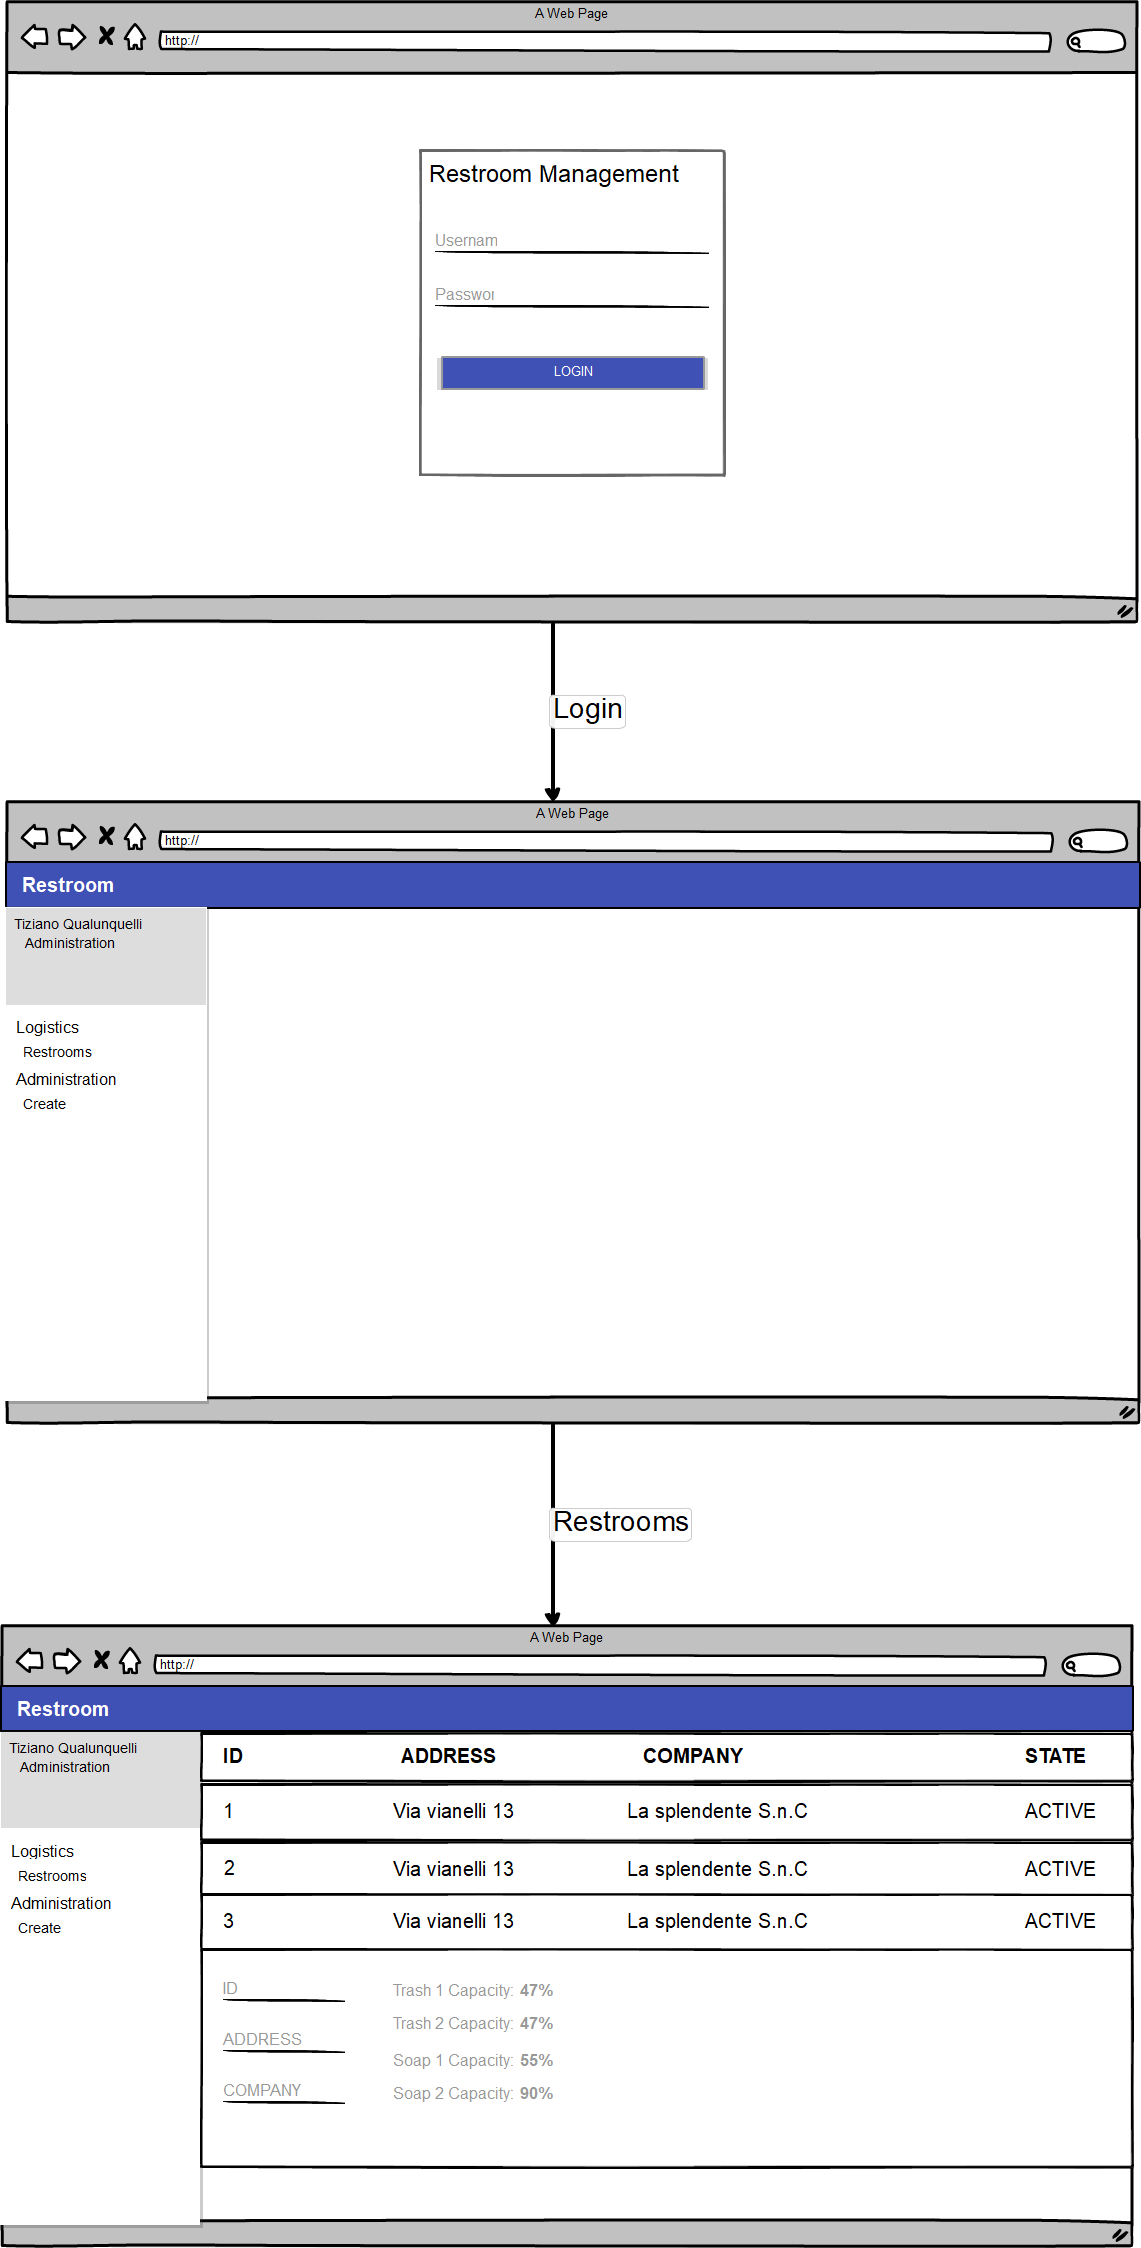
\includegraphics[scale=0.20]{img/mockup-manager.png}
  \caption{Mockup di \textit{manager}}
\end{figure}\\
A causa di una relativa familiarità a riguardo, il team di sviluppo si dedicherà ad uno stile \textit{Material Design} per tutte le schermate dell'applicazione.
\newpage
\subsubsection{Consumer}
\paragraph{Ambiente}
I requisiti esposti dal committente suggeriscono che \textit{consumer} debba essere un'applicazione a larga diffusione, facile da utilizzare e performante; in altre parole, un applicazione il cui utilizzo da un grande numero di persone (come cittadini e turisti) sia fondamentale.\\
Questa considerazione porta all'adozione di esperienze utente (UX) e soluzioni popolari, atte a non scoraggiare l'utente finale dall'utilizzo di \textit{consumer} a causa di un eccessiva complessità; considerato inoltre che l'applicazione sarebbe indirizzata all'utilizzo anche da parte di turisti, il team di sviluppo si adopererà per lo sviluppo di una \textit{mobile application}.\\
Tuttavia, ciò comporterebbe una lievitazione considerevole dei costi di sviluppo: seppur ridotta in termini di funzionalità, sarebbe necessario infatti sviluppare un applicazione per ogni sistema operativo \textit{mobile} presente sul mercato (\textit{Android} e \textit{iOS}).\\\\
A seguito di tali considerazioni, si è deciso di sviluppare \textit{consumer} come PWA (\textit{Progressive Web App}) garantendo così i seguenti vantaggi:
\begin{itemize}
\item Sviluppo multipiattaforma: essendo sostanzialmente un'applicazione web di nuova concezione con specifiche ottimizzazioni per il mondo mobile, una PWA è naturalmente multipiattaforma (è soltanto necessario un browser aggiornato per il suo utilizzo).\\
Questa caratteristica aiuterà a contenere i costi di sviluppo, in quanto sarà necessario sviluppare soltanto un'applicazione per tutti gli ambienti.
\item Distribuzione svincolata: applicazioni di questo genere permettono di essere installate localmente sul dispositivo, scaricando tutti le dipendenze richieste al loro funzionamento.\\%imitando in tutto e per tutto il comportamento delle più classiche app native distribuite attraverso \textit{store}.\\
Ciò permette di garantire all'utente una UX da applicazione nativa, pur rimanendo distribuita attraverso un semplice URL: una caratteristica senza dubbio utile per evitare tutti i vincoli dei tradizionali canali di distribuzione delle app (come gli \textit{store}).
\item Familiarità: come per \textit{manager}, le scelte progettuali di \textit{consumer} sono state parzialmente influenzate dallo \textit{skill set} preesistente del team di sviluppo. 
\end{itemize}
Come per l'applicazione di amministrazione, tuttavia, emergono delle problematiche relative alle tecnologie supportate dai dispositivi per la PWA: alcuni device infatti potrebbero rivelarsi incompatibili perché troppo datati.\\
Benché questo aspetto vada chiaramente in contrasto con la necessità di rendere \textit{consumer} utilizzata da un gran numero di utenti, i requisiti funzionali richiesti dal committente verranno rispettati nella loro totalità.\\
L'applicazione sarà comunque utilizzabile come un normale sito web: soltanto alcuni aspetti avanzati come l'installazione nativa, infatti, potranno risultare incompatibili.\newpage
\paragraph{Design}
La progettazione grafica di \textit{consumer} si è esclusivamente incentrata sulla creazione di un'app per dispositivi mobili focalizzata sulla semplicità e immediatezza.\\
Per il prodotto non sono state infatti previste versioni specificatamente studiate per PC desktop: considerato che la mobilità è un requisito fondamentale per il committente, si può dire che il suo utilizzo attraverso un personal computer sia quanto meno scoraggiato.\\
A causa della sua maggiore popolarità nel settore mobile verrà utilizzato uno stile \textit{Material Design} per tutte le schermate del prodotto; ciò aiuterà ad orientare meglio l'utente al primo approccio in quanto ricalcherà pattern oramai universali.
Di seguito viene presentato un primo mockup coerente con i punti precedentemente esposti:
\begin{figure}[h!]
\centering
  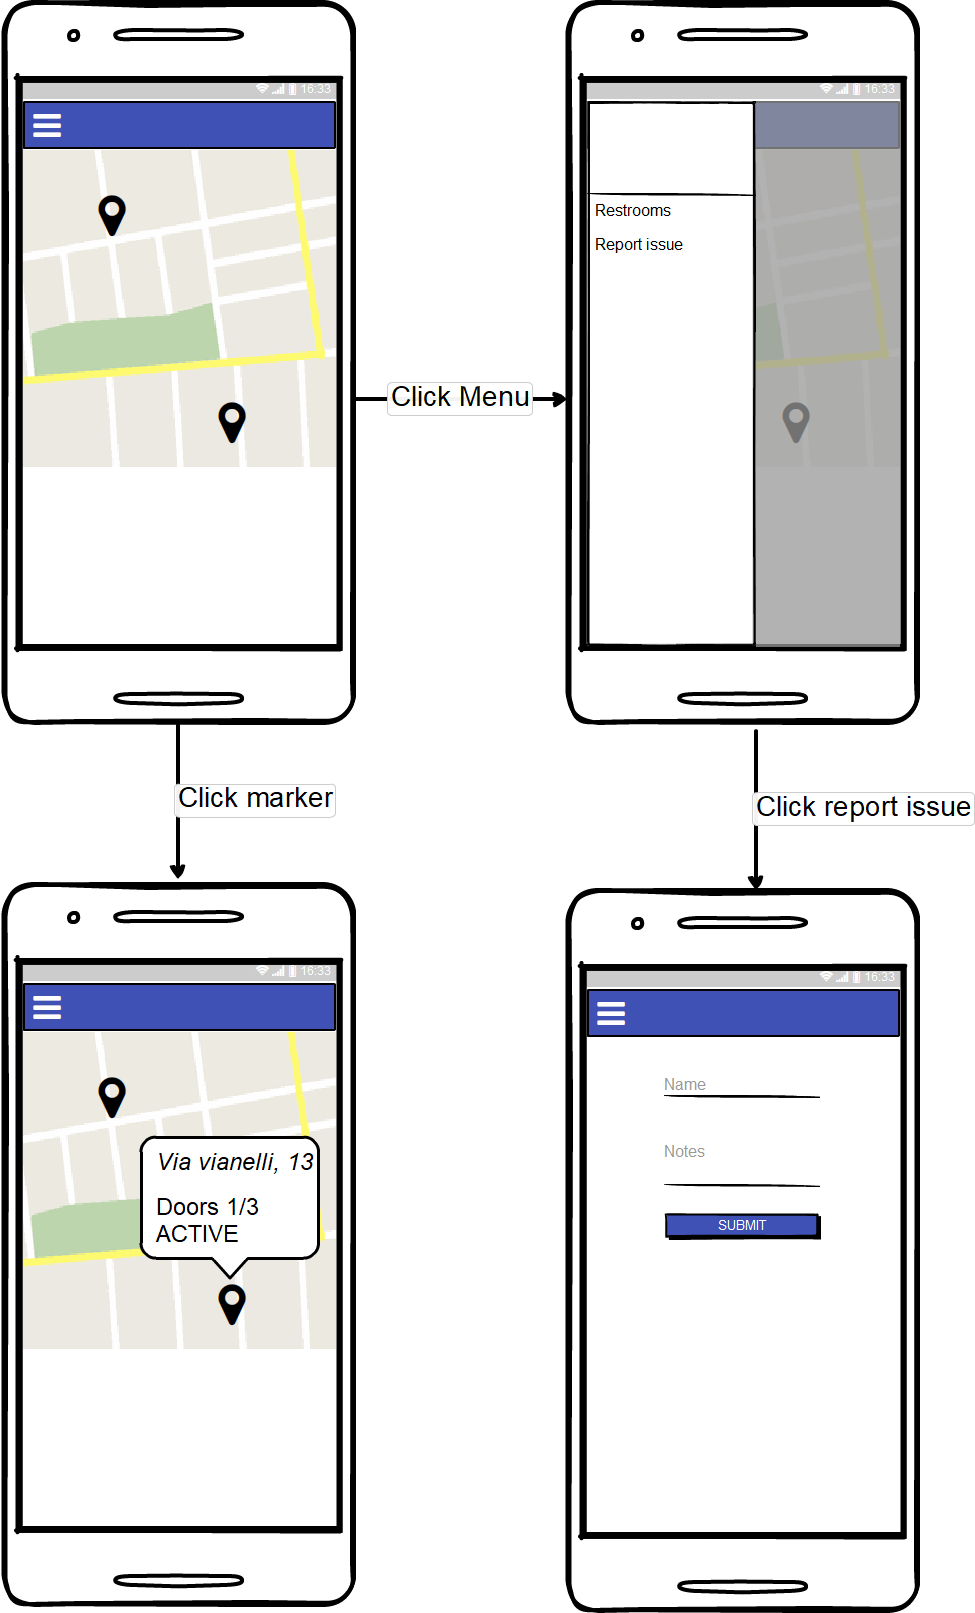
\includegraphics[scale=0.21]{img/mockup-consumer.png}
  \caption{Mockup di \textit{consumer}}
\end{figure}
\newpage
\subsection{Progettazione parte centrale}
La sezione di analisi dell'architettura ha evidenziato la necessità di creare un apposito \textit{server} RESTFul capace di fornire i dati richiesti dalle due applicazioni frontend (\textit{consumer} e \textit{manager}) e di raccogliere (e immagazzinare) i dati inviati dai singoli impianti installati.\\
Tali considerazioni profilano la realizzazione di 4 differenti entità:
\begin{itemize}
	\item Un web server per la fornitura delle risorse di \textit{manager}.
	\item Un web server per la fornitura delle risorse di \textit{consumer}.
	\item Un web server RESTFul dedicato alla gestione di tutte le richieste dei clients del sistema.\\Esso sarà l'unico con una connessione diretta con il DBMS.
	\item Un DBMS per archiviare le informazioni inviate dai client.
\end{itemize}
Le sottosezioni seguenti non affronteranno l'analisi progettuale dei web server per \textit{manager} e \textit{consumer}, in quanto considerate banali e non di particolare interesse.\\ 
Verrà però in primo luogo affrontata la parte di gestione dei dati: il DBMS.
\subsubsection{DBMS}
\paragraph{Tipologia}
Il particolare contesto in cui quest'applicazione è situata ha chiaramente influenzato la tipologia di DBMS scelto per l'archiviazione dati.\\
Al termine di alcune considerazioni. il team di sviluppo scelto un DBMS i tipo NOSQL con dati formattati BSON.\\Le motivazioni che hanno portato a questa scelta possono essere così riassunte: 
\begin{itemize}
\item Scalabilità orizzontale: \textit{MongoDb} basa la sua scalabilità sulla ridondanza piuttosto che sull'incremento di prestazione di un singolo server (\textit{scalabilità orizzontale}).\\
Ciò consentirà una notevole flessibilità della capacità del prodotto: sarà possibile infatti mantenere un numero di nodi ospitanti il DBMS coerenti con il numero di adozioni del sistema.
\item Semplicità: le interfacce RESTFul previste per la parte applicativa del progetto basano il loro input-output su dati in formato JSON.\\ Dato che \textit{MongoDB} supporta nativamente dati in formato BSON (un superset di JSON) ci si aspetta piena compatibilità e facilità di integrazione con il server di gestione di \textit{Manager} e \textit{Consumer}.
\item Budget ridotto: \textit{MongoDB} è fornito (anche per applicazioni commerciali) tramite licenza AGPL, che permette quindi un suo utilizzo gratuito a fronte di obblighi legali minimali.\\ Oltre a ciò, si ritiene interessante il cluster cloud che l'azienda fornisce per l'hosting del DBMS: i prezzi si sono rilevati competitivi e sicuramente migliori, in termini di costi finali e affidabilità, che una soluzione dedicata in azienda.
\end{itemize}
\paragraph{Struttura dati}

Al momento, è stata prevista una struttura piuttosto semplice contenente i dati del sistema, come raffigurato di seguito:
\begin{figure}[h!]
\centering
  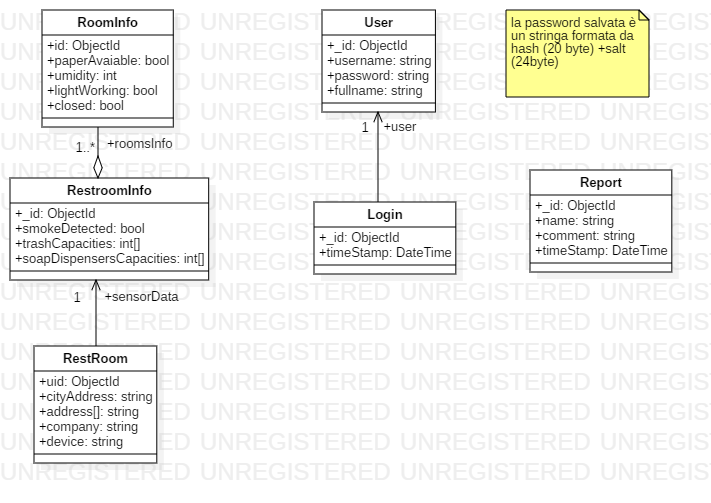
\includegraphics[scale=0.60]{img/class-diagram.png}
  \caption{Classi previste come \textit{Models} per il DBMS}
\end{figure}
\newpage
%parlare delle password hashate
\subsubsection{Server RESTFul}
A causa di una maggiore familiarità e compatibilità con le modalità di connessione delle applicazioni frontend, ogni endpoint pubblico del web server RESTFul supporterà unicamente comunicazioni di tipo POST.\\
Sebbene questo procedimento non si possa considerare accademicamente corretto (in genere sarebbe meglio progettare un server RESTFul affinché supporti una comunicazione di tipo CRUD) le risorse assegnate al team di sviluppo sono tali da non consentire altra scelta; considerando la notevole esperienza pregressa nello sviluppo di backend così improntati, inoltre, è evidente come questa sia l'unica strada percorribile per rientrare nei costi e nei tempi preventivati.\\

Il server prevede la costruzione di tre diversi controller contenenti gli endpoint pubblici del sistema, chiamati rispettivamente \textit{DevicesController}, \textit{ManagerController} e \textit{ConsumerController}.\\
Come facilmente intuibile dal loro nome, ognuno è dedicato a servire le richieste di una diversa parte \textit{logica} del sistema: \textit{DevicesController} per la parte locale (invio di dati dei sensori), \textit{ManagerController} per le utenze di \textit{manager} e \textit{ConsumerController} per le richieste di \textit{consumer}.\\\\
Ogni endpoint prevederà un'interfaccia dati standard per il valore di ritorno ricevuto, chiamato \textit{BaseResult}.\\
Tale interfaccia permette di stabilire un contratto di comunicazione tra i client e il server omogeneo in tutto il sistema: all'occorrenza esse possono essere ampliate (attraverso ereditarietà) per supportare altri tipi di payload.\\
\newpage
A titolo di esempio vengono presentate alcune classi utilizzate come valore di ritorno nelle API di \textit{ManagerController}:
\begin{figure}[h!]
\centering
  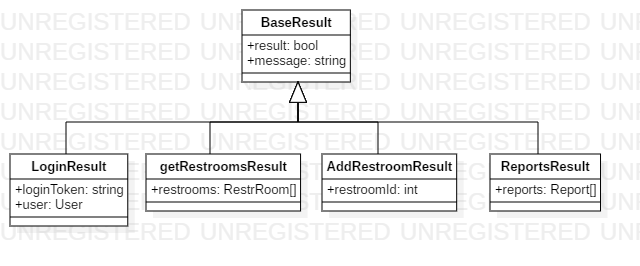
\includegraphics[scale=0.60]{img/classeBaseResult.png}
  \caption{Processo di registrazione di un nuovo impianto}
\end{figure}
\\Questo meccanismo fornisce una risposta standardizzata e semplificata delle operazioni effettuate: ciò facilità enormemente la loro gestione lato frontend.
\newpage
\subsection{Registrazione impianto}
\subsubsection{Configuratore} Per poter efficacemente spiegare il processo di registrazione di un nuovo impianto è necessario introdurre la figura del \textit{configuratore} (o \textit{installatore}) all'interno dell'architettura di sistema.\\
Questa figura ha il compito di installare fisicamente le \textit{smart restrooms} sparse sul territorio adoperandosi per la cablatura, configurazione e posizionamento di tutte le parti coinvolte.\\
Sarà responsabilità del \textit{configuratore}, infatti, il buon funzionamento del sistema locale a livello hardware; inoltre, trattandosi di apparecchiature delicate che richiedono una precisa configurazione, ogni intervento di manutenzione o potenziamento dell'infrastruttura dovrà essere eseguita da una persona certificata con questa qualifica. 
\subsubsection{Processo} 
La registrazione di un nuovo impianto è un processo che coinvolgerà interamente le tre parti costituenti l'architettura di \textit{smart-restrooms}: locale, applicativa (\textit{manager}) e server.\\
Ogni registrazione richiederà l'intervento di due tipologie di utenti, un \textit{configuratore} e un \textit{manager}, attraverso la seguente procedura:
\begin{enumerate}
\item Un utente \textit{manager}, attraverso l'apposita l'interfaccia del software, aggiunge un nuovo impianto specificando i dati obbligatori richiesti (come \textit{Company}, Address e \textit{CityAddress}).\\
Al termine di questa operazione ottiene un GUID che identifica il \textit{restroom} appena creato.
\item L'utente invia il GUID al \textit{configuratore}, che nel frattempo ha installato fisicamente il nuovo impianto.
\item Il \textit{configuratore} inserisce la chiave di identificazione (GUID) nel controller e installa la connettività di rete.
\end{enumerate}
Purtroppo, allo stato attuale, non è stato predisposto alcun metodo di distribuzione delle chiavi di identificazione tra \textit{manager} e \textit{configuratore}.\\
Si confida che, perlomeno in una prima istanza dell'applicazione, gli utenti utilizzino un mezzo di comunicazione a loro discrezione per scambiare i GUID appena creati.\\
Il processo sopra riportato può essere efficacemente schematizzato attraverso un diagramma \textit{Activity} presentato di seguito:
\begin{figure}[h!]
\centering
  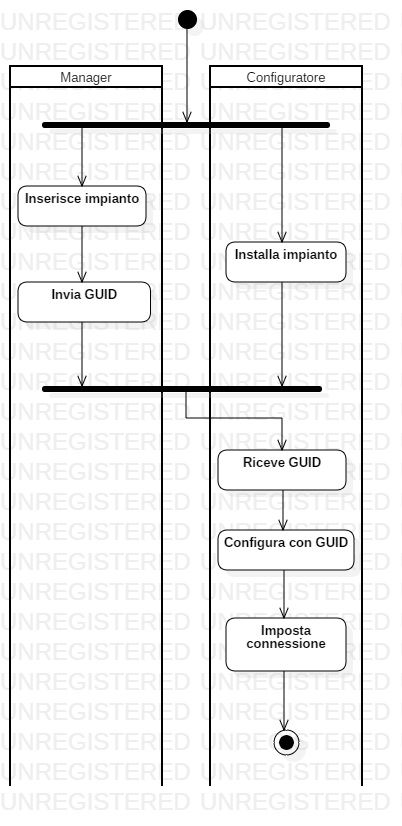
\includegraphics[scale=0.55]{img/activity_registration.png}
  \caption{Processo di registrazione di un nuovo impianto}
\end{figure}
\newpage
%----------------------------------------------------------------------------------------
%	IMPLEMENTAZIONE
%----------------------------------------------------------------------------------------

\section{Implementazione}\label{sec:implementazione}
\subsection{Implementazione parte locale}
Verranno di seguito illustrate le implementazioni per il software eseguito dal raspberry e il software eseguito dall'Arduino.
\subsubsection{Implementazione software Arduino}
Come riportato nella fase di progettazione, l'Arduino ha bisogno di un software leggero e computazionalmente poco complessso. Il software è scritto in C++; usa principalmente le librerie di base predisposte da Arduino e le librerie di terze parti per la lettura dei sensori digitali complessi.
\paragraph{Codice}
\subparagraph{Entrypoint}
[IMMAGINE DI CONCETTO SETUP AND LOOP]
L'entrypoint di un Arduino è determinato da file in estensione .cpp contenente due metodi:
\begin{itemize}
\item setup() Vero entrypoint del software, il metodo viene eseguito solo una volta, all'avvio.
\item loop() Metodo eseguito al termine del setup() e che viene rieseguito finché l'Arduino rimane alimentato.
\end{itemize}
Durante l'esecuzione del metodo di setup, verrà attivata la comunicazione attraverso la porta seriale [codice beginSerial()] e verranno inizializzati tutti i pin di input e output. Attraverso il file di intestazione con suffisso Mapping.h è possibile determinare quale pin è di input e quale è di output.
Al termine dell'inizializzazione verrà eseguito un rapido check sulle porte per determinare se il mapping è stato eseguito in maniera errata. Un mapping si definisce errato quando almeno uno dei pin è sia di input che di output.
[codice checkConflict()]
Se non ci sono conflitti, il setup termina e il dispositivo esegue il loop.\\
All'inizio di ogni loop, ci si chiede se è arrivato un messaggio di request dal raspberry. Se c'è allora viene consumata la prima string line disponibile. Su questa stringa viene effettuato un parsing preliminare per sapere di che comando si tratta e se riconosciuto si conclude il parsing in modo da ottenere i parametri necessari all'esecuzione del comando richiesto.
La struttura del messaggio di richiesta è la seguente:
MethodToCall,pin,status
 Infine, se necessario, l'Arduino manda indietro la risposta con l'esito o risultato del comando. [codice loop.switch()]

\subparagraph{Mapping}
Affinché il mapping lato codice sia effettuato con cura è necessario creare un file header contenente tre metodi principali:
\begin{itemize}
\item getInputMapping(int value) Metodo che, preso il numero di pin come parametro, restituisce il nome del sensore, ad esso mappato, che ha lo scopo di inviare dati al sistema locale.
\item getOutputMapping(int value) Metodo che, preso il numero di pin come parametro, restituisce il nome del sensore, ad esso mappato, che ha lo scopo di ricevere dell'input da Arduino per un possibile cambio di stato.
\item evaluateMappingType(int value) Metodo che, preso il numero di pin come parametro, restituisce il tipo di sensore collegato a quel pin (esempio se è digitale o analogico).
\subparagraph{Lettura di pin di input}
Se la request include il comando di lettura di un pin, prima di leggere il suo stato, bisogna conoscere la tipologia di sensore collegato. Generalmente le librerie Arduino permettono di conoscere lo stato del pin (HIGH o LOW), ottimo per sensori digitali semplici come gli interruttori; se invece è necessario leggere lo stato di un sensore digitale complesso come il dht, la libreria standard di Arduino non è più sufficiente. La community di Arduino mette a disposizione librerie di terze parti per i sensori al momento più conosciuti. In questo caso quindi è necessario installare le librerie di terze parti e cambiare il comportamento della lettura del pin in base al sensore ad esso collegato. [codice readFromPin(int pin)]
\end{itemize}
\subsubsection{Implementazione software Raspberry}
[Mappa concettuale software raspberry]
\paragraph{Caratteristiche}
Come anticipato in parte nel capitolo di progettazione, il software che viene eseguito sul raspberry verrà scritto in Java 8. Questa scelta è stata influenzata dalle proprietà principali che Java 8 offre:
\begin{itemize}
\item Un grande supporto dalla community di Java
\item Numerose librerie di terze parti disponibili
\item Il recente inserimento del paradigma alla programmazione funzionale e programmazione reattiva
\item Possibilità di eseguire Java su tutte le architetture più diffuse
\end{itemize}
\subparagraph{Librerie di terze parti}
Per l'uso e la sincronizzazione di librerie di terze parti si è scelto di usare Maven.
Tra le librerie third-party si prevede almeno l'utilizzo delle seguenti:
\begin{itemize}
\item RXTX.dll per la comunicazione con Arduino
\item rxjava per implementare le componenti reattive
\item gson per la costruzione della stringa Json da inviare al server centrale
\item httpclient per implementare la classe di connessione al server centrale
\end{itemize}


\paragraph{Codice}
Il codice d'implementazione rispecchia concettualmente quello che è stato già definito in fase progettuale. Verrà descritto quindi il codice relativo alla componente sensori e il codice relativo al manager.
\subparagraph{Sensori}
L'interfaccia ISensor si occupa di esporre i metodi basilari che ogni sensore virtuale deve poi implementare; estende l'interfaccia Runnable in modo da integrare la logica dei 'Java.Thread' al suo interno. ISensor verrà implementato parzialmente da AbstractSensor, una classe astratta che incorpora il comportamento principale che ogni sensore deve avere.
L'abstractSensor deriva anche dalla classe Observable; implementerà quindi un ulteriore comportamento, la sua parte reattiva. Grazie all'implementazione dell'Observable in AbstractSensor è possibile modificare lo stato di tutti gli oggetti di tipo Observer che si sono iscritti.
\begin{lstlisting}
	protected boolean updateObserver(EntrySet entry)
	{
		if (!this.connectedObserver.isPresent())
			return false;
		this.connectedObserver.get().onNext(entry);
		return true;
	}
\end{lstlisting}
L'abstractSensor viene a sua volta implementato da ArduinoSensor, una seconda classe astratta che implementa a sua volta la classe Observer. In questo modo ArduinoSensor è in grado non solo di aggiornare possibili subscribers ma anche di iscriversi ad un'altro Observable e di reagire ai suoi aggiornamenti. Grazie a questa implementazione, l'ArduinoSensor reagisce alle risposte da parte dell'Arduino e può iscriversi ad un altro ArduinoSensor per reagire alle variazioni di stato del sensore virtuale a cui si è iscritto.
Le classi finali sono ArduinoReadingSensor e ArduinoWritingSensor.
Il comportamento di queste due classi sono simili; la differenza sostanziale sta nel fatto che l'ArduinoReadingSensor, una volta che riceve le informazioni dall'Arduino, aggiorna il Manager mentre l'ArduinoWritingSensor ha il solo scopo di cambiare lo stato dei pin relativi ai Sensori fisici di output (come il pin di un led); entrambi le classi sfruttano il Manager per comunicare con l'Arduino.
La ragione principale per cui si è creato un livello di astrazione così profondo è quella di tenere alta la libertà di usare, in futuro, un dispositivo differente da Arduino per la gestione fisica dei sensori. 
\subparagraph{Manager}
Il manager è composto da 3 macro parti:
\begin{itemize}
\item RestroomSM: responsabile del coordinamento di tutte le componenti
\item IOComm: responsabile della comunicazione tra manager-arduino e sensori virtuali-arduino
\item RestClient: responsabile della comunicazione tra manager e server
\end{itemize}
L'\textbf{IOComm} è la classe responsabile alla comunicazione tra Raspberry e Arduino e implementa l'interfaccia Observer per reagire alle risposte da parte di Arduino. Per inizializzare un oggetto di questa classe è richiesta la lista di porte seriali a cui i vari Arduino sono fisicamente connessi al Raspberry. 
Durante l'inizializzazione, la classe interroga ogni Arduino connesso per ricevere la lista delle mappature dei sensori fisici utilizzati e crea le strutture necessarie a memorizzare queste mappature e legarle concettualmente all'Arduino interrogato. Per ogni stringa di mappatura ricevuta dagli Arduino, l'IOComm inizializza i sensori virtuali di tipo ArduinoSensor passando loro informazioni utili al loro funzionamento; le principali informazioni sono:
\begin{itemize}
\item relative all'Arduino fisico a cui concettualmente appartiene come la porta seriale e il numero di pin a cui il sensore fisico è cablato.
\item relative alle proprietà funzionali del sensore virtuale come il delay che ci deve essere tra un'interrogazione all'Arduino e un'altra.
\end{itemize}
Una volta conclusa l'inizializzazione è possibile comunicare con l'Arduino con l'ausilio di due metodi di classe esposti:
\begin{itemize}
\item sendWriteRequestToArduino(), metodo che serve a cambiare lo stato di un pin di un Arduino
\item sendReadRequestToArduino(), metodo che serve a leggere lo stato di un pin di un Arduino
\end{itemize}
Il \textbf{RestClient} è una classe che permette al Raspberry di comunicare ad un server con tecnologia Rest. Durante la sua inizializzazione, viene richiesto l'indirizzo URL a cui il Raspberry si connetterà e vengono impostate le metodologie di comunicazione, come l'utilizzo dell'http post con struttra dei messaggi in Json.
La classe espone il metodo sendData() che prende come parametro l'informazione strutturata da spedire.
Il metodo serializza l'informazione in formato Json, crea la struttura di request e response e spedisce il messaggio. E' possibile conoscere l'esito dell'operazione tramite il metodo .getStatusLine().getStatusCode() della struttura di response; il risultato del metodo sopra citato è un intero che rappresenta il codice di stato http. Se l'esito è andato a buon fine, lo status code sarà uguale a 200. All'interno della response inoltre c'è un oggetto Json deserializzabile in un oggetto di classe RestResponse che riporta il risultato dell'operazione di business e un possibile messaggio.
\textbf{RestroomSM} (Restroom sensor manager) è la classe principale del software; essa implementa sia le funzioni di Observable che le funzioni di Observer. Questa classe serve a collegare i sensori virtuali con l'IOComm, si collega al RestClient e tiene in memoria una struttura dati ben definita da aggiornare e/o inviare al Server durante il suo ciclo di vita.
Durante la sua inizializzazione, il RestroomSM recupera, dal file di configurazione dell'applicazione, tutte le informazioni necessarie a inizializzare correttamente l'IOComm, il RestClient e la struttura dati. Inoltre il manager mappa il nome delle porte ai dispositivi arduino e i dispositivi arduino alle strutture dati. Infine,se necessario , crea le dipendenze tra i vari ArduinoSensors.
Il RSM espone due funzioni:
\begin{itemize}
\item Start() Abilita tutti i sensori virtuali ad esso collegati
\item Stop() Ferma tutti i sensori virtuali ad esso collegati
\end{itemize}
Una volta avviatosi, il cuore della classe è rappresentata dalla funzione onNext() metodo derivato da Observer.
Questo metodo viene chiamato dai vari sensori virtuali come Observable e ha il compito di smistare le informazioni per aggiornare la struttura dati. Al termine dello smistamento dei dati, viene chiesto l'invio della struttura dati tramite l'ausilio della classe RestClient.
\newpage
\subsection{Implementazione parte Applicativa}
\subsubsection{Manager}
\paragraph{Caratteristiche}
Il capitolo di progettazione di \textit{manager} prevedeva lo sviluppo di una applicazione web di tipo SPA caratterizzata da una certa complessità, facilità di manutenzione e scalabilità.\\
Con queste premesse, il team di sviluppo ha deciso di adottare \textit{Angular} come framework per lo sviluppo dell'applicazione.\\\\
Adottato specificatamente nella versione 6+, \textit{Angular} è un set di librerie frontend open-source studiate appostiamente per una creazione agevole e strutturata di SPA; creata e mantenuta tutt'ora direttamente da \textit{Google}, questo framework si posiziona al primo posto per popolarità per la creazione di progetti enterprise web.\\
Benché infatti si presti anche allo sviluppo di prodotti di ridotta complessità, lo sviluppo attraverso \textit{Angular} è caratterizzato da una curva di apprendimento ripida e dalla necessità di scrivere molto codice \textit{boilerplate} per sviluppare funzionalità semplici; benché queste caratteristiche lo rendano capace di strutturare adeguatamente progetti frontend complessi, molti team di sviluppo lo ritengono uno strumento troppo potente (e difficile) per le loro necessità.\\
Concludendo, questo \textit{framework} è stato scelto rispetto ad altre librerie popolari (come \textit{React} o \textit{Vue}) per i seguenti motivi:
\begin{itemize}
\item \textit{Angular} fornisce direttamente funzionalità utili allo sviluppo di SPA come \textit{Dependency Injection}, \textit{AJAX}, gestione token ecc.\\
I suoi principali competitor, essendo librerie e non \textit{framework}, richiedono l'integrazione con dipendenze di terze parti (esponendo il prodotto a una minore mantenibilità).
\item Grazie a una suddivisione in moduli e sottomoduli e al supporto della \textit{Dependency Injection
}, un applicazione scritta attraverso \textit{Angular} permette di scalare la sua complessità in maniera nettamente migliore rispetto al processo non strutturato e completamente in mano al programmatore tipico delle altre librerie.
\item Avendo già sviluppato prodotti di una certa complessità attraverso questo framework, il team di sviluppo si è dimostrato particolarmente efficiente.
\end{itemize}
L'applicazione è stata scritta in Typescript, super-set di Javascript che permette di scrivere codice per applicazioni web attraverso il paradigma ad oggetti.\\
La sua notevole somiglianza con il linguaggio c\#, inoltre, ha reso lo sviluppo del lato server più semplice (dato che è stato scritto in asp.net core).
\paragraph{Librerie}
Segnaliamo qui le dipendenze esterne degne di nota necessarie al funzionamento del progetto:
\begin{itemize}
\item \textit{Angular Material:} libreria per interfacce utente basate sul \textit{material design} e largamente supportata dalla comunità dell'omonimo \textit{framework}.\\
Gran parte degli artefatti grafici presente nell'applicazione (tabelle, notifiche, inputs) sono disegnati grazie all'utilizzo di questa versatile libreria.
\item \textit{Ngx local storage:} libreria che consente di archiviare valori nella cache del browser attraverso una serie di strategie (indexedDB, local storage ecc.).\\
Viene unicamente utilizzata per mantenere in memoria il \textit{loginToken}.
\end{itemize}
\paragraph{Codice}
In \textit{Angular}, ogni componente visiva principale dell'applicazione viene modellata come un \textit{Component}, cioè un costrutto composto da un \textit{controller} (cioè una parte nella quale risiede la logica del componente: funzioni, variabili, hooks) e un \textit{template} (cioè, in ambito web, un sezione di HTML e CSS).\\
Questo elemento è indispensabile per specificare singole funzionalità o parti riusabili dell'applicazione, grazie alla sua sintassi precisa e inedita nel mondo dello sviluppo frontend.\\
Considerato inoltre che i progetti \textit{Angular} devono passare attraverso una procedura di compilazione (o, più precisamente, transpilazione) dei file sorgente, si può capire come lo sviluppo di applicazioni particolarmente complesse venga agevolata: ogni file sarà esente da errori di compilazione (anche grazie all'uso del paradigma OOP) e il progetto avrà una struttura chiara e definita formalmente.
\newpage
Come primo esempio viene presentato il \textit{component} dedito alla login utente:
\begin{lstlisting}

import { Component } from '@angular/core';
@Component({
  selector: 'app-login',
  templateUrl: './login.component.html',
  styleUrls: ['./login.component.scss']
})
export class LoginComponent {
// constructor(loginService: LoginService...) {}

  login(form: NgForm) {
    this.loginService.login(form.v.username, form.v.password).subscribe(success => {     
     
        if (success) 
          this.router.navigate(['']);
        else
          this.snack.open("Wrong username or password", null, {panelClass: 'loginSnackbar'});
    });
  }}
\end{lstlisting}
\phantom{\\}
Si possono notare i seguenti punti d'interesse: 
\begin{itemize}
\item Importazione delle dipendenze attraverso la parola chiave \textit{import}.\\
Questo meccanismo si può considerare simile all'inclusione di package presente in C\# e Java.
\item Dichiarazione del componente attraverso il decoratore \textit{@Component}.\\ 
Un decoratore non è altro che un meccanismo per estendere le funzionalità di una classe attraverso il framework.
\item Subscription del form di login: ogni tentativo di login da parte dell'utente richiamerà la lambda mostrata.\\
In caso di successo, viene spostata la navigazione utente alla home della webApp.\\
In caso contrario, viene mostrata una notifica di errore grazie alla libreria \textit{Angular Material}.
\end{itemize}
Un altra sezione di particolare interesse sono le \textit{Routes} e le \textit{Guards}.\\
Le prime vengono utilizzate dal framework per impostare gli \textit{url} a cui l'applicazione dovrà rispondere: attraverso di esse sarà possibile specificare quale \textit{Component} mostrare e con quali parametri.\\
Le seconde, invece, possono essere associate a \textit{routes} per determinare la loro attivazione in base alle condizioni inserite: \textit{manager} utilizza delle \textit{guards} per prevenire che utenti non autenticati possano accedere a sezioni protette dell'applicazione.\\\\
Un esempio di tale guard viene presentata di seguito:
\begin{lstlisting}

import { Injectable } from "@angular/core";
@Injectable()
export class AuthGuard implements CanActivate {
//  constructor(storage: LocalStorage...) {}

    canActivate() {
        if (!this.loginService.user == null)
            return true;

        return this.storage.getItem('loginToken').
        pipe(concatMap(loginToken => {
            if (loginToken == null) {
                this.router.navigate(['/login']);
                return of(false);
            }
            return this.loginService.loginByToken(loginToken);
        }));
    }
}
\end{lstlisting}
Anche qui vengono evidenziati i seguenti punti d'interesse:
\begin{itemize}
\item In modo analogo al componente descritto in precedenza, in questa classe viene specificato un decoratore (\textit{@Injectable}) per donare alla classe uno specifico comportamento.
\item L'implementazione dell'interfaccia \textit{CanActivate} serve a specificare la tipologia di \textit{Guard} adottata: in questo caso si tratterà della più semplice, cioè per determinare la validità di una certa \textit{Route} richiesta (attraverso il metodo \textit{canActivate()}).
\item \textit{this.storage.getItem()} rappresenta è un esempio di utilizzo della libreria \textit{Ngx local storage} descritta nella sezione precedente: in questo caso mostrato il reperimento di un \textit{loginToken} di sessione.\\
Qualora il token non esista (e quindi l'utente non sia autenticato) allora si rimanda l'applicazione all'indirizzo di login.\\
In caso contrario la \textit{Route} viene accettata e fatta proseguire.
\end{itemize}
\newpage
\subsubsection{Consumer}
\paragraph{Caratteristiche}
Il capitolo di progettazione di \textit{consumer} evidenzia la necessità di sviluppare \textit{consumer} come un'applicazione di tipo PWA.\\
Questa scelta è stata dovuta principalmente ai suoi più rapidi tempi di sviluppo rispetto a una normale app nativa; date le ridotte risorse a disposizione, il team di sviluppo è sempre stato propenso a ridurre i costi, dove possibile.\\
Pertanto, per evitare di investire tempo nella formazione di personale per l'utilizzo di tecnologie specifiche per PWA, è stato deciso di utilizzare \textit{Angular} per lo sviluppo di \textit{Consumer}.\\\\
La natura poliedrica di questo framework, infatti, permette di aggiungere il supporto alle \textit{Progressive Web apps} attraverso dei semplici moduli e pochi file di configurazione aggiuntivi: gran parte del funzionamento dell'app, infatti, verrà gestita da \textit{Angular} (ad esempio, non sarà necessario sviluppare direttamente un \textit{service worker}).\\
Infine, anche in questo caso verrà utilizzato \textit{Typescript} come linguaggio di programmazione
\paragraph{Librerie}

Segnaliamo qui le dipendenze esterne degne di nota necessarie al funzionamento del progetto:
\begin{itemize}
\item \textit{Angular Material:} anche in questo caso è stata utilizzata questa libreria per il disegno e la gestione delle interfacce utente.\\
Utilizzare la stessa dipendenza nei due prodotti si è dimostrato utile nel risparmiare sui costi di sviluppo, dato che la tecnologia adottata era divenuta familiare.
\item \textit{Angular Google Maps Core:} i requisiti esposti dal committente rendono chiaro il desiderio di mostrare una \textit{gmap} per orientare l'utente nella ricerca di un bagno pubblico; ciò è stato possibile grazie all'inclusione della libreria \textit{Angular Google Maps Core} all'interno del progetto.\\
Per poter avviare il servizio, inoltre, è stato necessario fornire all'applicazione un apposita chiave di identificazione.

\end{itemize}
\paragraph{Codice}
Dato il suo sviluppo in \textit{Angular} come il già analizzato \textit{manager}, non verranno qua analizzate le modalità di costruzione delle funzionalità di \textit{consumer}, che si possono infatti considerare pressoché simili.\\
Inoltre, dato che gran parte del codice necessario per rendere \textit{consumer} una PWA non è stato sviluppato direttamente dal team ma generato automaticamente dal framework (attraverso un tool di transpilazione chiamato \textit{angular-cli}) il suo approfondimento non si ritiene meritevole di interesse.\\\\
Tuttavia, si ritiene importante analizzare nel dettaglio le modalità con le quali è stato possibile mostrare a schermo una \textit{gmap} interattiva con l'utente, in particolare il lato \textit{template} che è stato tralasciato nella precedente sezione.\\
Innanzitutto, \textit{Angular} consente di effettuare un \textit{binding} (cioè un collegamento) tra una variabile presente nel \textit{controller} e il rispettivo \textit{template} attraverso due modalità: \textit{box casing} (cioè racchiudendo l'attributo a cui assegnare una variabile tramite i caratteri []) oppure tramite \textit{double brackets} (cioè racchiudere il nome della variabile assegnata a un certo attributo tramite i caratteri \{\}).\\\\
Ad esempio, l'implementazione della \textit{gmap} nel componente è stato effettuato attraverso un binding di tipo \textit{box casing}, come mostrato di seguito: 
\begin{lstlisting}[style=htmlcssjs]

<agm-map [latitude]="userPosition[0]" [longitude]="userPosition[1]"
[zoom]="14">

  <agm-marker *ngFor="let restRoom of restRooms; let i = index"
              (markerClick)="restRoomSelected(restRoom)"
              [latitude]="restRoom.address[0]"
              [longitude]="restRoom.address[1]">

    <agm-info-window>
      <app-marker-detail [restRoom]="restRoom"></app-marker-detail>
    </agm-info-window>
  </agm-marker>
</agm-map>
\end{lstlisting}
\newpage
Oltre al \textit{binding}, si possono notare i seguenti punti d'interesse:
\begin{itemize}
	\item \textit{agm-map}, \textit{agm-marker} e \textit{agm-info-window} sono componenti esterni forniti dalla libreria \textit{Angular Material}.\\ Come qualsiasi altro elemento HTML, possono essere  istanziati semplicemente specificando il loro nome nel template. 
	\item Il componente \textit{agm-marker} viene istanziato tante volte quanti sono gli elementi presenti nell'array \textit{restRooms} del \textit{controller} (grazie alla direttiva \textit{*ngFor}).\\ Visivamente, ciò permette di disegnare i \textit{marker} descritti nell'analisi dei requisiti e mostrati nel mockup della fase di progettazione.
	\item \textit{app-marker-detail} invece corrisponde a un componente scritto dal team di sviluppo: esso servirà a rappresentare il contenuto esposto (\textit{popover}) al click di un \textit{marker}.
\end{itemize}
\newpage
\subsection{Implementazione parte centrale}
\subsubsection{Server}
\paragraph{Caratteristiche}
La progettazione della parte centrale del sistema ha previsto la creazione di un generico server RESTFul in grado di rispondere alle richieste delle altre entità coinvolte nel sistema.\\
Dato che i requisti del committente non hanno dato alcuna indicazione sul suo ambiente di destinazione e la progettazione non ha individuato vincoli in tal senso, il team di sviluppo ha optato per una soluzione multipiattaforma, gratuita e opensource come \textit{ASP.NET Core}.\\
Questo framework di sviluppo backend è stato creato e tutt'ora direttamente mantenuto da \textit{Microsoft}, in futura sostituzione del più classico ambiente ASP.NET, che dalla sua introduzione (circa 2016) ha ricevuto una crescente popolarità come soluzione general-purpose backend.\\
Comunque, le motivazioni che hanno spinto il team di sviluppo a scegliere questa tecnologia possono essere così riassunte: 
\begin{itemize}
\item Le elevate prestazioni garantite dal framework (sopratutto in situazioni di elevato carico da parte di host multipli) lo rendono perfettamente adatto al carico di lavoro previsto del progetto.
\item La natura multipiattaforma di \textit{ASP.NET Core} consente una notevole flessibilità sull'ambiente di hosting di destinazione.\\
Ciò consentirà una scelta più ampia e concorrenziale e, pertanto, un maggiore ritorno economico del sistema.
\item La stretta vicinanza con l'ambiente di sviluppo delle applicazioni frontend (scritte in Typescript) ha migliorato l'efficienza generale del team.\\
Data la notevole somiglianza dei linguaggi C\# e Typescript, infatti, non è stato necessario assegnare risorse nella formazione degli sviluppatori.
\end{itemize}
Precisamente, il server implementato in \textit{ASP.NET Core} è di tipo \textit{Web Api}, cioè specifico per la creazione di server RESTFul.\\
La prossima sezione si dedicherà all'analisi delle API implementate più rilevanti a fini di studio.
\paragraph{API}
Strutturalmente, il server è composto da una serie di file chiamati \textit{controller} che separano le API dedicate di ogni parte logica del sistema.\\
Ogni controller è caratterizzato da una radice di API diversa: ad esempio tutti gli endpoint di \textit{ConsumerController} sono nella forma:
\begin{center}
\textit{https://public-restrooms/api/consumer/api-name}
\end{center}
Come inoltre già previsto dalla fase di progettazione, tutte le interfacce esposte del server prevedono un input nel metodo HTTP POST, con un \textit{payload} che varia in base all'endpoint selezionato.\\
Tuttavia, sebbene i payload di ingresso cambino radicalmente per ogni endpoint esposto, il valore di ritorno di essi è prevedibile grazie alla derivazione di una classe base chiamata \textit{BaseResult}, che qui brevemente esponiamo:
\begin{lstlisting}

public abstract class BaseResult
{
    public bool Result { get; set; }
    public string message { get; set; }
}
\end{lstlisting}
Questo meccanismo fornisce a tutti i client del sistema un contratto di comunicazione per ogni possibile API esposta dal server.\\ 
Ne consegue che l'implementazione delle chiamate HTTP è notevolmente semplificata e coerente.\\\\
Viene qui mostrato un primo esempio di endpoint del server che adotta questo meccanismo, cioè un' interfaccia atta alla registrazione di nuove \textit{restRooms} inviate dall'utente:
\newpage
\begin{lstlisting}
[Route("addRestroom")]
[HttpPost]
public ActionResult<AddRestroomResult> AddRestroom(AddRestroomData addRestroomData)
{
    AddRestroomResult result = new AddRestroomResult();
    if (!ValidUserSession())
            return result;
        
    IMongoCollection<Models.RestRoom> restroomsCollection = _db.GetCollection<Models.RestRoom>("Restroom");
    
    Models.RestRoom newRestroom = new Models.RestRoom(addRestroomData.guid, addRestroomData.address.Split(','), addRestroomData.cityAddress, addRestroomData.company, "");
    restroomsCollection.InsertOne(newRestroom);

    result.Result = true;
    return result;    
}
\end{lstlisting}
Da questo esempio si evidenziano i seguenti punti fondamentali:
\begin{itemize}
	\item Trattandosi di un API per app \textit{manager}, la prima operazione che viene effettuata è il controllo della sessione utente corrente attraverso il metodo \textit{ValidUserSession()}.\\
	Ciò avviene ricercando il \textit{loginToken} inviato tra gli headers di ogni richiesta nel DBMS: qualora esista un record di login recente contenente il \textit{loginToken} inviato, allora la richiesta verrà autenticata.
	\item Grazie al sistema di \textit{Dependency Injection} di \textit{ASP.NET Core}, viene recuperata la sessione di connessione con il DBMS corrente (attraverso il metodo \textit{GetCollection()}).
	\item Viene infine ricostruito il dato inviato dall'utente in un formato compatibile con il modello di DB e inviato al DBMS.\\ Come ultimo step, viene notificato all'utente la buona riuscita dell'operazione.
\end{itemize}
\subsubsection{DBMS}
\paragraph{Caratteristiche}
La fase di progettazione relativa al DBMS ipotizzava l'utilizzo di un database NOSQL con dati in formato BSON.\\
Sebbene esista un ampia scelta di prodotti per database con queste caratteristiche, il team di sviluppo ha scelto \textit{MongoDb} come prodotto commerciale a supporto dell'applicazione a seguito delle seguenti considerazioni: 
\begin{itemize}
\item \textit{Maturità}: la progettazione di un sistema di notevole complessità e consistente flusso dati richiede l'utilizzo di tecnologie affidabili e ben supportate.\\
Considerato che nessun membro del team di sviluppo annovera esperienze di utilizzo di database NOSQL, si è scelto di non cimentarsi nell'adozione di prodotti meno conosciuti sul quale vi sarà minore supporto e documentazione.
\item \textit{Integrazione}: sono disponibili gratuitamente dei set di librerie per integrare \textit{ASP.NET Core} con \textit{MongoDB}.\\
Ciò ha permesso ovviamente di velocizzare i tempi di sviluppo in quanto la connessione con il DBMS ha richiesto una configurazione minimale.
\item \textit{Hosting}: sono disponibili soluzioni di hosting gratuite (fornite direttamente dalla \textit{MongoDb Inc.}) per l'utilizzo del DBMS su cloud.\\
Oltre che essere semplici da utilizzare, non hanno vincoli di durata e le prestazioni generali sono accettabili per un utilizzo iniziale del sistema; è chiaramente possibile aumentare adeguatamente le prestazioni del \textit{Tier} in qualsiasi momento.
\end{itemize}
Come anticipato, si è deciso di delegare la gestione del DBMS al servizio cloud offerto gratuitamente dalla compagnia di MongoDB.\\
Precisamente, l'offerta \textit{Free Tier} offre un hosting cloud basato con queste caratteristiche:
\begin{itemize}
\item Hosting fornito da AWS situato a Francoforte.
\item 512Mb di spazio di storage massimo.
\item RAM del cluster condivisa con altre utenze.
\end{itemize}
Sebbene queste caratteristiche possano sembrare un po' limitanti, si confida in un loro upgrade immediato qualora il prodotto abbia successo.
\paragraph{Connessione}
L'utilizzo di tecnologie ben supportate e recenti come \textit{MongoDB} e \textit{ASP .NET Core} ha facilitato molto la connessione al database, rendendo minimi gli sforzi per la sua attuazione.\\
Tutti le operazioni di input-output avvengono infatti attraverso classi c\# (racchiuse nel namespace \textit{Models}) che sanciscono la tipologia di oggetti salvati nel DB: la libreria di \textit{MongoDB} si occuperà poi di trasformare automaticamente tali classi in formato JSON.

\begin{lstlisting}
// Ottenimento, grazie alla Dependency injection, di un istanza di connessione con il DB
IMongoCollection<Models.RestRoom> restroomsCollection = _db.GetCollection<Models.RestRoom>("Restroom");
// Inserimento di una nuova restroom all'interno del database
Models.RestRoom newRestroom = new Models.RestRoom(restroom.guid, restroom.address.Split(','), restroom.cityAddress, restroom.company, "");
restroomsCollection.InsertOne(newRestroom);

\end{lstlisting}
\newpage
%----------------------------------------------------------------------------------------
%	TESTING E PERFORMANCE
%----------------------------------------------------------------------------------------

\section{Testing e performance}
\subsection{Performance parte Locale}
\subsubsection{Parte hardware}
La longevità dell'impianto elettrico dipende dalla qualità dei sensori utilizzati. Tuttavia, data la progettazione semplificata e l'installazione non invasiva, è possibile sostituire qualsiasi tipo di guasto elettronico.
\subsubsection{Parte software}
Molto più preoccupante la stabilità del sistema software; data la scarsità di risorse disponibili per lo sviluppo di tutto il progetto, si è tralasciata una sezione molto importante del progetto: la gestione degli errori. In un primo rilascio dell'intero progetto infatti la gestione degli errori è stata ridotta all'osso. Questo significa che per qualsiasi malfunzionamento l'applicazione lato raspberry potrebbe rompersi; occorre quindi un riavvio manuale da remoto dell'applicazione per ristabilire il corretto funzionamento del sistema.
\newpage
\subsection{Performance parte applicativa}
Nell'ambito di applicazioni RESTful le performance finali si possono considerare dipendenti da due fattori:
\begin{itemize}
\item \textit{Tempo richiesta:} è il tempo che intercorre tra l'invio l'invio della richiesta e la ricezione della sua risposta dal server.
\item \textit{Tempo renderizzazione:} è il tempo impiegato per la processione dei dati ricevuti e per la loro effettiva visualizzazione a schermo.
\end{itemize}
Quindi, un utente percepisce la responsività di un'applicazione RESTful come la \textit{somma} del tempo di richiesta e il tempo di renderizzazione per una specifica azione; tutte le successive analisi presenti in questa sezione pertanto terranno conto di questa suddivisione.
\subsubsection{Manager}
Come già analizzato nei capitoli precedenti, \textit{Manager} è un applicazione studiata per il monitoraggio di un numero di impianti consistente ad aggiornamento continuo.\\
Innanzitutto, partendo dall'analisi fornitaci dal \textit{Webpack Bundle Analizer}\cite{bundleAnalyzer}, si può osservare come il \textit{footprint} dell'applicazione sia molto ridotto (circa \textit{200kb gzipped}); ciò consentirà un caricamento immediato delle risorse dell'applicazione (anche nel caso in cui l'utente rifiuti qualsiasi tipo di cache web sul sistema).
\begin{figure}[h!]
\centering
  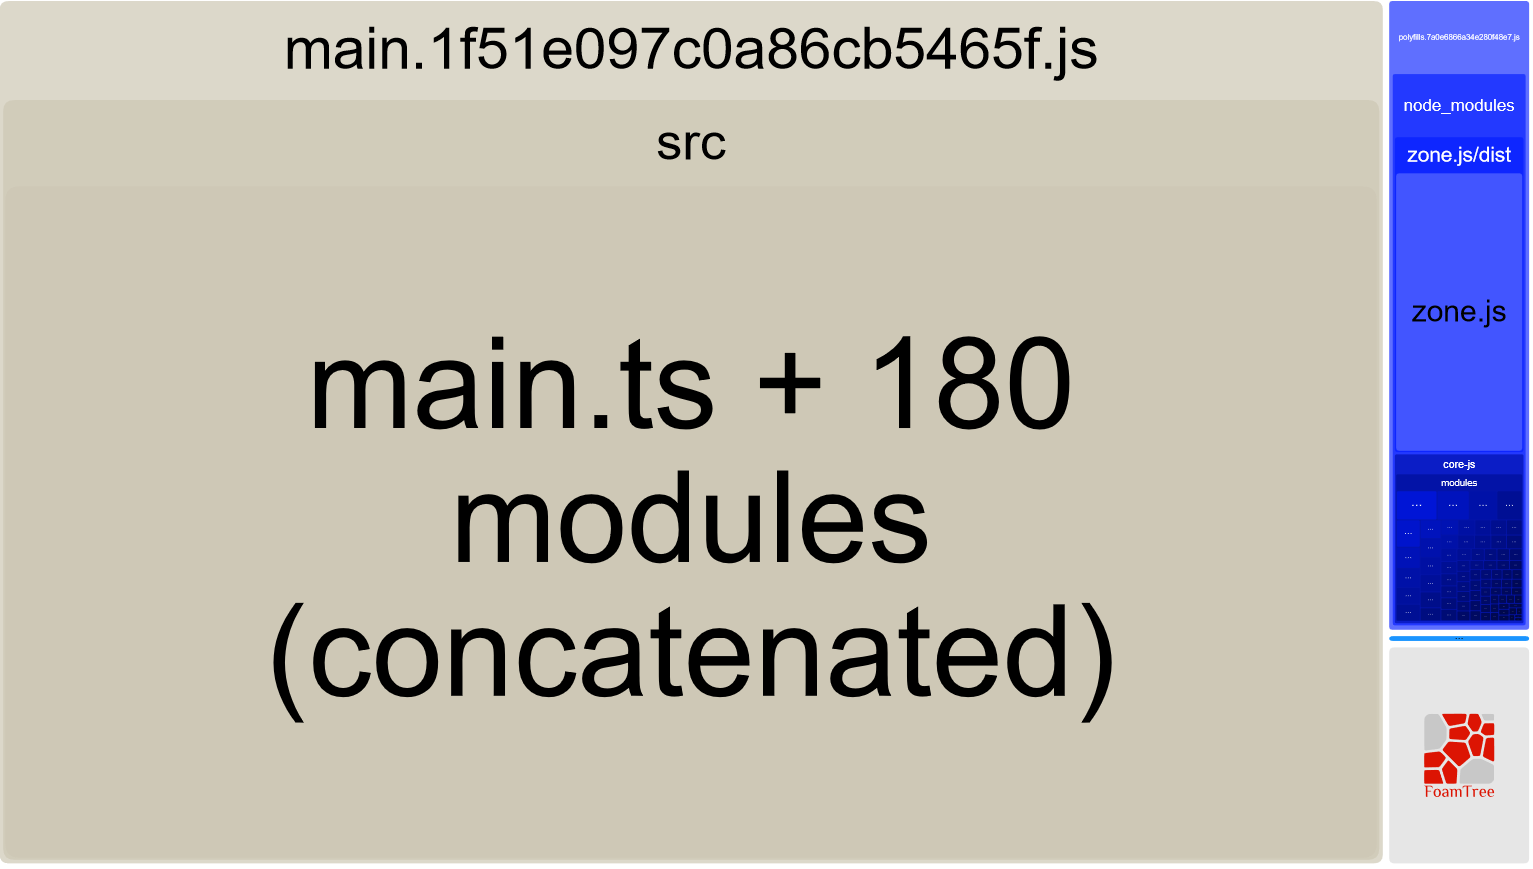
\includegraphics[scale=0.18]{img/footprint-manager.png}
  \caption{Composizione del bundle di produzione di \textit{manager}}
\end{figure}
\newpage
In seguito, è stato misurato il tempo che l'applicazione ha impiegato per ottenere dati aggiornati dei \textit{restrooms} presenti su DB (per un totale di 6), grazie all'utilizzo delle funzioni \textit{console.time()} e \textit{console.timeEnd()} nativamente presenti in ES6.

\begin{lstlisting}
export class RestroomsListService {

  constructor(private httpClient: HttpClient) { }

  getRestrooms() {
    console.time("downloadTime");
    return this.httpClient.post("api/manager/getRestrooms", {}).pipe(map((restrooms: any) => {
      console.timeEnd("downloadTime");
      return restrooms.restrooms;
    }));
  }
}
\end{lstlisting}
Tale test ha portato ai seguenti risultati:
\begin{table}[h]
\begin{tabular}{|c|c|}
\hline
\textbf{Richiesta N°} & \textbf{Tempo Totale}  \\ \hline
1 & 98,56 ms  \\ \hline
2 & 119,51 ms \\ \hline
3 & 83,07 ms  \\ \hline
4 & 112,06 ms \\ \hline
5 & 111,16 ms \\ \hline
\end{tabular}
\end{table}\\
per una latenza media risultante di \textit{104,6 ms.}\\
Dato che tale risultato non si può definire particolarmente performante, si è proceduto ad effettuarne un'analisi approfondita per individuarne cause e possibili soluzioni.\\\\
Circa il 55\% della latenza è da imputare alla connessione con il DB \textit{mongoDb Atlas}, che ricordiamo essere basato su un cluster gratuito AWS situtato a Francoforte, con memoria RAM condivisa e 512Mb di spazio dedicato.\\
È chiaro pertanto che, in questo caso, l'utilizzo di una soluzione gratuita ha inciso in maniera rilevante sulle prestazioni del sistema: in fase di produzione si raccomanda pertanto la scelta di un cluster con almeno RAM dedicata e preferibilmente situato nei pressi della locazione del server centrale.\\\\
Il server, invece, è stato ospitato sulla rete domestica di \textit{Stefano Belli} utilizzando un suo PC personale (composto da una CPU Intel i5 4690k, 8gb di RAM e SSD Sata III, con sistema operativo  Windows 10 Pro x64): non si tratta di quindi di un hardware \textit{ad hoc} dedicato a ospitare server per SPA, ma un normale PC con memoria condivisa per altri programmi ad uso personale.\\Anche in questo caso, pertanto, si dovrebbe operare sull'infrastruttura per migliorare le performance generali.\\\\
Infine, si è pensato di effettuare una build in modalità \textit{Release} del server, in modo da sfruttare tutte le ottimizzazioni che tale processo garantisce (ad esempio ignorando completamente il debugging).\\
Ciò ha permesso di ridurre sensibilmente il tempo di esecuzione totale di ogni richiesta, come si può evincere dalla tabella sottostante:
\begin{table}[h]
\begin{tabular}{|c|c|}
\hline
\textbf{Richiesta N°} & \textbf{Tempo Totale}  \\ \hline
1 & 64,45 ms  \\ \hline
2 & 80,05 ms \\ \hline
3 & 74,58 ms  \\ \hline
4 & 71,83 ms \\ \hline
5 & 72,40 ms \\ \hline
\end{tabular}
\end{table}\\
per una latenza media risultante di \textit{72,66 ms.}\\\\
Come premesso poco sopra, questi tempi sono da considerare come \textit{Tempi Totali}, cioè al netto della renderizzazione a schermo (e quindi come somma di \textit{Tempo Richiesta} e \textit{Tempo Renderizzazione}).\\
Ulteriori analisi hanno determinato come il solo \textit{Tempo di Richiesta} incida per il 70\% sul tempo totale.
\newpage
Ciò viene anche dimostrato dall'analisi delle richieste effettuate dal \textit{Chrome Developers Tools}:
\begin{figure}[h!]
\centering
  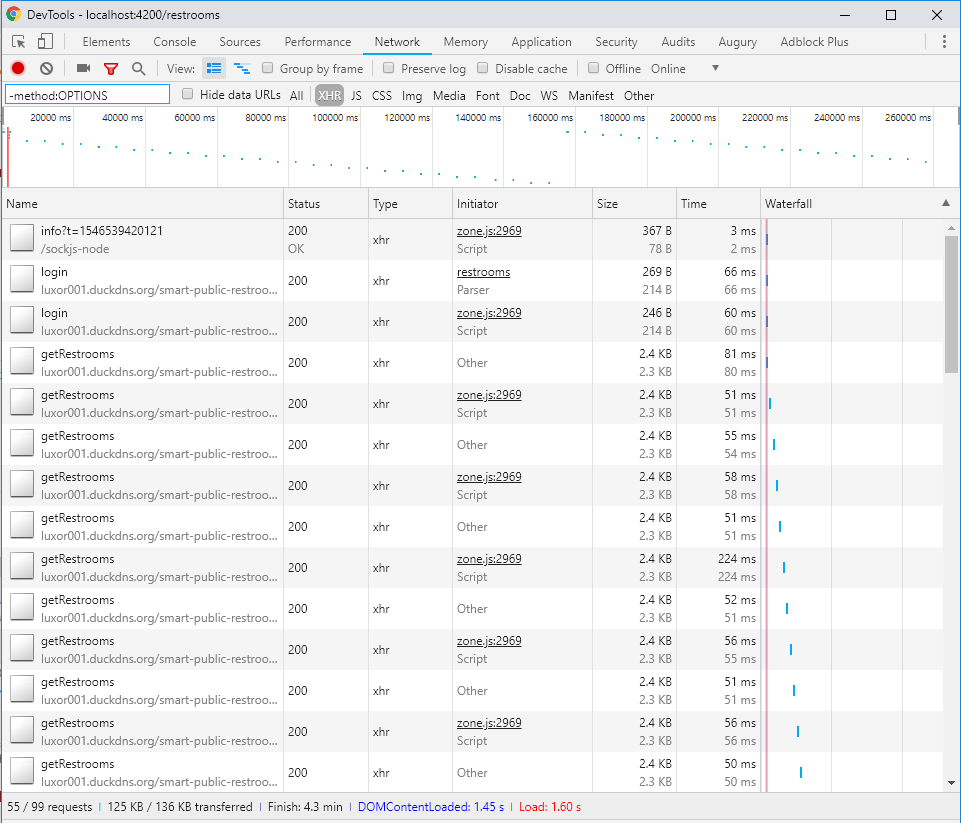
\includegraphics[scale=0.60]{img/network-timings.png}
  \caption{Tempi di richiesta secondo \textit{Chrome Developers Tools}}
\end{figure}

\subsubsection{Consumer}
\textit{Consumer} e \textit{Manager} utilizzano le stesse infrastrutture server e DB e pertanto le prestazioni della PWA si possono dire molto simili a quelle della SPA; dato che l'applicazione è al momento molto contenuta, non si rilevano criticità a livello di performance rispetto a \textit{Manager}.
%----------------------------------------------------------------------------------------
%	ANALISI DI DEPLOYMENT SU LARGA SCALA
%----------------------------------------------------------------------------------------

\section{Analisi di deployment su larga scala}
\subsection{Parte Applicativa}
\textit{Smart Public Restrooms} è un sistema che riteniamo essere molto scalabile e in generale poco esoso in termini di risorse necessarie: come vedremo, infatti, i volumi dati coinvolti per un cliente di una certa dimensione sono tutto sommato contenuti e comunque gestibili.\\
Innanzitutto, poniamo qualche stima sul volume dati coinvolto per un cliente con circa 2000 impianti in gestione: 

\begin{itemize}
\item \textit{Richieste/minuto}: Ogni sistema invia dati al server centrale ogni 5 secondi, per un totale di 12 volte al minuto.\\
Con un numero di impianti da gestire come sopra (2000), si arriverebbe a circa 24000 cicli di aggiornamento su DB al minuto.
\item \textit{Spazio/impianto}: L'\textit{Average Size} dei documenti della tabella \textit{Restroom} (contenente i dati essenziali dell'impianto, come nome, indirizzo e gli ultimi dati della sensoristica) è pari a 500 byte.\\
Con 2000 impianti totali lo spazio occupato su DB si attesterebbe a circa 1MB.
\item \textit{Bandwidth/impianto}: Il payload di un aggiornamento di un impianto tipico (con 3 celle e 3 pattumiere di servizio) si aggira sui 500 byte.\\
Con 2000 impianti totali l'infrastruttura di rete del server dovrà riuscire a supportare $~200Kb/s$ in upload e $\frac{N}{5}Mb/s$ in download, dove N è il numero di clients \textit{Manager} connessi.
\end{itemize}
Queste semplicistiche stime ci danno un'idea piuttosto chiara delle risorse necessarie per il mantenimento di un sistema \textit{Smart Public Restroom}; un cliente con circa 2000 impianti attivi non dovrebbe avere grossi problemi nel gestire tali traffici dati, eccezion fatta per la \textit{Bandwidth} necessaria in download.\\
Allo stato attuale, infatti, ogni client \textit{Manager} richiede al server tutte le \textit{Restrooms} disponibili su db ogni 5 secondi, comportando per un ognuno di essi l'ottenimento di circa 1Mb di dati dal server periodicamente: ciò rallenta sia l'applicazione \textit{frontend} che l'intero server.\\
La soluzione a questo problema è quella di restringere il numero di \textit{Restrooms} ottenute periodicamente dall'applicazione, ad esempio attraverso l'uso di filtri configurabili dall'utente.\\\\
Supponiamo ora che la software house che ha sviluppato \textit{Smart Public Restrooms} decida di gestire in prima persona tutti i \textit{Restrooms} dei suoi clienti (che supponiamo essere 10, ognuno con qualche migliaio di impianti): il sistema dovrà mantenere delle buone prestazioni (sia in termini di \textit{efficiency} che di \textit{fault tolerance}) nonostante il numero enorme di impianti a cui dovrà far fronte.\\\\
Data la sua natura centralizzata, l'elemento più a rischio in questa configurazione è sicuramente il server di gestione del sistema: se da un lato le sue prestazioni possono rimanere accettabili con tecniche di scalabilità verticale, rimane comunque una fonte importante di \textit{Single Point of Failure} \textit{(SPoF)}.\\
Una possibile soluzione a questo problema è quella di applicare tecniche di \textit{Loose Coupling} sui server, in grado quindi di costruire una rete composta una serie di nodi indipendenti sulla quale distribuire le richieste avanzate dai clients.\\
Nell'ambito dell' \textit{Internet Information Services} \textit{(IIS)} di \textit{Microsoft} (cioè attraverso le tecnologie utilizzate per la realizzazione del server di \textit{Smart Public Restrooms}) ciò è possibile attraverso la configurazione di nodi  \textit{Application Request Routing} (\textit{ARR}), cioè moduli di routing che redirigono il traffico di rete in base a particolari algoritmi di \textit{load balancing}, header HTTP e variabili d'ambiente.
\begin{figure}[h!]
\centering
  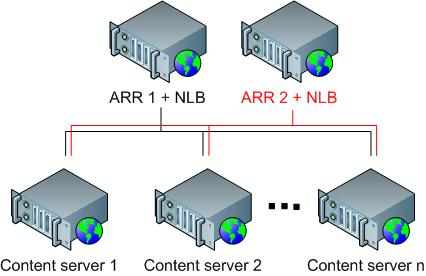
\includegraphics[scale=0.80]{img/ARR.png}
  \caption{Architettura con ARR+NLB}
\end{figure}
\newpage
In generale, architetture di questo tipo consentono una buona \textit{Avaiability} e \textit{Scalability} del sistema, ma rendono difficoltoso sincronizzare gli accessi al DB tra i vari nodi della rete.\\
Fortunatamente, gli aggiornamenti inviati dagli impianti di \textit{Smart Public Restrooms} si possono considerare stateless e indipendenti, in quanto ogni richiesta temporizzata fa riferimento a un singolo impianto ed è quindi impossibile avere conflitti in scrittura su DB.\\\\
Inoltre, prevediamo il DBMS sia perfettamente in grado di scalare in modo adeguato alle esigenze dell'applicazione: la sua natura NoSQL e la semplicità dei dati contenuti ben si prestano a tecniche di \textit{scalabilità orizzontale} come lo \textit{Sharding}, che prevediamo adatto a scenari \textit{write-intensive} come questo.\\
In questo scenario, tuttavia, ci raccomandiamo di affidarci ai cluster  forniti da \textit{MongoDb} per l'hosting del DBMS, in quanto già integrati all'interno dell'applicazione e sicuramente comprovati come affidabili per questo tipo di utilizzi (ad esempio, si prevede che \textit{MongoDb} abbia adeguati strumenti di \textit{Disaster Recovery}).\\\\
Qualora queste strategie di \textit{Scalability} non siano sufficienti (o siano troppo esose), si ritiene possibile aumentare progressivamente la frequenza di aggiornamento delle \textit{Restrooms}: la maggioranza dei dati raccolti non hanno necessità di essere tempestivamente notificate all'utente, eccezion fatta per l'allarme "fumo".\\ 
In tal caso si può studiare un meccanismo di invio di \textit{push notifications} o messaggi SMS (tramite modulo GMS installato negli impianti) direttamente agli utenti di \textit{Manager}.\\\\
Infine, raccomandiamo l'utilizzo di servizi come \textit{CloudFlare} per la \textit{DDoS Mitigation} e più in generale per l'ottenimento di un sufficiente livello di \textit{Overload Protection}.
\subsection{Parte Locale}

\newpage
%----------------------------------------------------------------------------------------
%	PIANO DI LAVORO
%----------------------------------------------------------------------------------------
Il progetto appena presentato è stato interamente realizzato da un team di due persone, \textit{Stefano Beli} e \textit{Andrea Vecchiotti}.\\
La divisione dei compiti è stata netta e basata sull'affinità di ogni membro del gruppo di lavoro:
\begin{itemize}
	\item \textit{Stefano Belli} si è occupato della creazione e gestione della parte \textit{applicativa} e \textit{server}.\\
	Più dettagliatamente, si è occupato della progettazione e sviluppo del server scritto in \textit{ASP.NET Core} e della relativa connessione con il DBMS.\\
	Si è inoltre incentrato sulla realizzazione del database in MongoDB e del relativo deploy su cloud \textit{Atlas} come descritto nel capitolo 6.\\
	Infine, si è dedicato alla realizzazione delle applicazioni \textit{manager} e \textit{consumer} e della relativa progettazione.
	\item \textit{Andrea Vecchiotti} ha preso in carico lo sviluppo del lato locale; si è occupato quindi della realizzazione del progetto lato hardware e nella progettazione e sviluppo dei software eseguibili su arduino e raspberry, interazione tra le due componenti e la comunicazione tra raspberry e il server centrale.
\end{itemize}
Nella stesura di questa documentazione di progetto ogni membro si è dedicato al suo specifico ambito di lavoro; altre sezioni generiche (come la qui presente) si possono considerare soggette a un lavoro collettivo.\\\\
Per quanto riguarda le tempistiche, \textit{Stefano Belli}  ha riportato:
\begin{itemize}
\item Circa 6 giorni/uomo per lo sviluppo del frontend dell'app \textit{consumer}.
\item Circa 18 giorni/uomo per lo sviluppo del frontend dell'app \textit{manager}.
\item Circa 10 giorni/uomo per lo sviluppo (e deploy) della parte server.
\item Circa 25 giorni/uomo per la stesura della relazione.
\end{itemize}

\textit{Andrea Vecchiotti} ha riportato invece:
\begin{itemize}
\item Circa 20 giorni/uomo per lo sviluppo del software eseguibile su raspberry
\item Circa 5 giorni/uomo per lo sviluppo del software eseguibile da arduino
\item Circa 6 giorni/uomo per la progettazione e montaggio dell'hardware
\item Circa 5 giorni/uomo per la stesura della relazione
\end{itemize}
\newpage


%----------------------------------------------------------------------------------------
%	CONCLUSIONI
%----------------------------------------------------------------------------------------

\section{Conclusioni}
Questo progetto rappresenta un valido caso di studio per la messa in pratica delle principali nozioni di \textit{Smart City e tecnologie mobili} viste durante il corso di Sistemi Autonomi presieduto dal prof. Maio.\\
Innanzitutto, è stato progettato un sistema di monitoraggio completo e vicino a un contesto reale: sono stati coperti aspetti che spaziano dalle modalità di installazione degli impianti alla copertura delle esigenze degli utenti finali.\\
Il sistema si è rivelato sia economico nella sua realizzazione (in termini di costi dei materiali e tempistiche di sviluppo) che flessibile per eventuali sviluppi futuri: l'adozione di tecnologie come \textit{MongoDB} e la creazione di SPA con \textit{Angular} sono solo alcune delle scelte architetturali che riteniamo importanti per garantire al sistema la capacità di scalare gradualmente con la sua adozione in massa.\\\\
Tuttavia, la sua possibile resa economica pone alcuni interrogativi, che derivano dal fatto che \textit{Smart Public Restrooms} è un prodotto particolare adatto soltanto a una ristretta cerchia di clienti: le dimensioni delle aziende target devono essere tali infatti da porre la necessità di ridurre i costi di manutenzione dei bagni pubblici offerti nei propri servizi.\\
Si ritiene improbabile, pertanto, che il sistema da noi progettato possa di fatto essere il \textit{core business} di un'ipotetica Startup, perché i tempi necessari per approdare nel mercato possono essere importanti; ciò è anche aggravato dal fatto che esistono già alcune soluzioni sul mercato comparabili con \textit{Smart Public Restrooms}.\\
Il suo sviluppo può essere tuttavia interessante per Software House di una certa dimensione e già affermate nel settore (con quindi altri introiti derivanti da altri prodotti); in quest'ottica, per aumentare i ricavi si potrebbe offrire direttamente anche il servizio di manutenzione e monitoraggio dei servizi pubblici dei clienti.\\\\
Ciononostante, \textit{Smart Public Restrooms} rimane un sistema flessibile con interessanti potenzialità; riteniamo di aver ideato un prototipo di un prodotto realisticamente piazzabile sul mercato e didatticamente rilevante.
\newpage


%----------------------------------------------------------------------------------------
%	APPENDICE
%----------------------------------------------------------------------------------------

\newpage


%----------------------------------------------------------------------------------------
%	RIFERIMENTI BIBLIOGRAFICI
%----------------------------------------------------------------------------------------
\addcontentsline{toc}{section}{Riferimenti bibliografici}
\begin{thebibliography}{9}
\bibitem{articolo1}
\textit{$http://www.salute.gov.it/resources/static/uffici/DPR_26marzo1980n327.pdf$}

\bibitem{KooBathroom} 
Dan D. Kooa, John J. Leea, Aleksei Sebastiania, Jonghoon Kimb \\
\textit{An Internet-of-Things (IoT) system development and
implementation for bathroom safety enhancement}.\\
Procedia Engineering 145 ( 2016 ) 396 – 403 

\bibitem{txt2clean}
\textit{https://www.txt2clean.com/}

\bibitem{restroomalert}
\textit{https://www.restroomalert.com/}

\bibitem{restroom-management-system}
\textit{http://www.advantech.com/iretail-hospitality/solutions/detail/restroom-management-system}

\bibitem{onvation}
\textit{https://www.kcprofessional.com/en-us/workplacesolutions/onvation}

\bibitem{bundleAnalyzer}
\textit{https://www.npmjs.com/package/webpack-bundle-analyzer}

\end{thebibliography}

%----------------------------------------------------------------------------------------

\end{document}